% Creating a simple Title Page in Beamer
\documentclass[aspectratio=169, xcolor={dvipsnames}, 10pt, brazil]{beamer}
\usepackage{tikz}
\usetikzlibrary{shapes.geometric, arrows}

% Define styles
\tikzstyle{startstop} = [rectangle, rounded corners, minimum width=2cm, minimum height=0.6cm, text centered, draw=black, fill=yellow!30, font=\tiny]
\tikzstyle{process} = [rectangle, minimum width=2cm, minimum height=0.6cm, text centered, draw=black, fill=blue!30, font=\tiny]
\tikzstyle{response} = [rectangle, minimum width=1.1cm, minimum height=0.6cm, text centered, draw=black, fill=red!30, font=\tiny]
\tikzstyle{arrow} = [thick,->,>=stealth]

% Pacotes
\usepackage{lipsum}
\usepackage{graphicx}
\usepackage{color}
\usepackage[table]{xcolor}
\usepackage{tikz}
\usepackage{tcolorbox}
\usepackage{amsmath}
\usepackage{amsfonts}
\usepackage{amssymb}
\usepackage{mathrsfs}
\usepackage{mathtools}
\usepackage{enumitem} 
\usepackage{float}
\usepackage[utf8]{inputenc}	
\usepackage[portuguese]{babel}
\usepackage{caption}


% Theme choice:
\usetheme{CambridgeUS}

% Cores personalizadas
\definecolor{PROFMATgreen}{RGB}{0, 138, 163}
\definecolor{UFTgreen}{RGB}{0, 137, 124}
\definecolor{UFTblue}{RGB}{0, 84, 132}
\definecolor{UFTyellow}{RGB}{253, 185, 46}
\definecolor{UFTgray}{RGB}{132, 134, 136}

% Ativar numeração de tabelas
\setbeamertemplate{caption}[numbered]

% Definir novo estilo de item com quadrado verde
\setlist[itemize,1]{label=\textcolor{UFTgreen}{\rule{1ex}{1ex}}}

\setbeamercolor*{structure}{bg=UFTgreen,fg=black}

\setbeamercolor*{palette primary}{fg=black,bg=PROFMATgreen}
\setbeamercolor*{palette secondary}{fg=white,bg=UFTblue}
\setbeamercolor*{palette tertiary}{fg=black,bg=UFTgreen}
\setbeamercolor*{palette quaternary}{fg=white,bg=black}

\setbeamercolor{section in toc}{fg=black,bg=white}
\setbeamercolor{alerted text}{fg=white}

\setbeamercolor*{item}{fg=PROFMATgreen}

\setbeamercolor{block title}{bg=UFTgreen,fg=white}
\setbeamercolor{block body}{bg=UFTgray!10,fg=black}

\setbeamercolor{titlelike}{fg=white, bg=UFTblue}
\setbeamercolor{frametitle}{bg=UFTgray!20,fg=UFTgreen}



\setbeamertemplate{background}{
    \parbox[c][\paperheight][c]{\paperwidth}{
        \vfill
        
\includegraphics[width=\paperwidth,height=\paperheight,keepaspectratio]{img/modelo/bakcground.png} 
        \vfill
    }
}


% Customizar a página de título
\setbeamertemplate{title page}{
    \vbox{}
\begin{minipage}{0.2\linewidth}
        \centering
        % 
\includegraphics[width=0.6\linewidth]{img/modelo/uft-brasao.png}
    \end{minipage}
    \hfill
    \begin{minipage}{0.2\linewidth}
        \centering
        % 
\includegraphics[width=0.6\linewidth]{img/modelo/profmat-logo.png}
    \end{minipage}
    
    %\vfill
    \vskip1em\par
    \begingroup
        \centering
        \begin{beamercolorbox}[sep=8pt,center,shadow=true,rounded=false]{title}
            \usebeamerfont{title}\inserttitle\par%
            \ifx\insertsubtitle\@empty%
            \else%
                \vskip0.25em%
                {\usebeamerfont{subtitle}\usebeamercolor[fg]{subtitle}\insertsubtitle\par}%
            \fi%
        \end{beamercolorbox}%
        \vskip1em\par
        \begin{beamercolorbox}[sep=6pt,center]{author}
            \usebeamerfont{author}\insertauthor
        \end{beamercolorbox}
        \vskip0.2em\par
        \begin{beamercolorbox}[sep=5pt,center]{advisor}
            \usebeamerfont{institute} \advisorname
        \end{beamercolorbox}
        \vskip0.2em\par
        \begin{beamercolorbox}[sep=5pt,center]{institute}
            \usebeamerfont{institute}\insertinstitute
        \end{beamercolorbox}
        \vskip0.2em\par
        \begin{beamercolorbox}[sep=5pt,center]{date}
            \usebeamerfont{institute}\insertdate
        \end{beamercolorbox}
        \vskip0.5em\par
    \endgroup
    \vfill
}


% Remover bordas arredondadas dos blocks
\makeatletter
\setbeamertemplate{blocks}[default] % Isso remove o arredondamento
\makeatother


% Pacotes de citações
% ---

\usepackage[alf,abnt-etal-text=it,abnt-repeated-author-omit=yes,abnt-etal-list=0,abnt-etal-cite=3,abnt-emphasize=bf]{abntex2cite}	% Citações padrão ABNT



\setbeamercolor{bibliography entry author}{fg=black}
\setbeamertemplate{bibliography item}{\newblock}


\setbeamertemplate{frametitle continuation}{}

% Redefinir o separador para um traço
% Redefinir o separador
\captionsetup[figure]{labelformat=simple, labelsep=endash, textformat=period, font=footnotesize}
\captionsetup[table]{labelformat=simple, labelsep=endash, textformat=period, font=footnotesize}


% Redefine espaçamento antes e depois da legenda em figuras e tabelas
\captionsetup[figure]{aboveskip=2pt, belowskip=0pt}
\captionsetup[table]{aboveskip=2pt, belowskip=0pt}


% Define uma penalidade alta para a hifenização
\hyphenpenalty=10000
\tolerance=10000


% Personalizando o estilo da tabela de conteúdos
\setbeamertemplate{section in toc}[sections numbered]
\renewcommand{\thesection}{\textcolor{PROFMATgreen}{\arabic{section}}}
\renewcommand{\thesubsection}{\textcolor{PROFMATgreen}{\arabic{section}.\arabic{subsection}}}

\setbeamersize{text margin left=0.8cm, text margin right=0.8cm}

\usetikzlibrary{shadows,positioning,fit}
\usetikzlibrary{arrows.meta}
\usetikzlibrary{shapes.geometric}
\usepackage{graphicx}
\usepackage{amsmath, amssymb}
% \documentclass{beamer}
\usepackage{tcolorbox}
\usepackage{xcolor}
\usepackage{enumitem}
\definecolor{myblue}{HTML}{0057B7}
\definecolor{mygreen}{HTML}{007F5F}
\definecolor{myorange}{HTML}{F77F00}
\definecolor{myred}{HTML}{D62828}
% Informações do documento
\title[]{Tree of Thoughts Prompting}
% \author[]{Md. Siam Ahamed }
% \author[]{Md. Siam Ahamed }
\institute[]{Department of Computer Science and Engineering,BUET}
\date{}

% Definir o nome do orientador
\newcommand{\advisorname}{\textbf{Presentor:}\\ Md. Siam Ahamed \\ Al Shahriar Alif\\Imdadul Hasan}




\begin{document}

% Slide (frame) de título
\begin{frame}
    \titlepage
\end{frame}


% Sumário
\begin{frame}[t]
    \frametitle{Summary }
     \tableofcontents
\end{frame}

% Seção de Introdução
\section{Introduction}

\begin{frame}{What is prompting ??}

    \begin{itemize}
		\item Prompting involves offering some kind of guidance or encouragement to elicit a response, action, or thought from the person or system being prompted.
	\item \textcolor{gray!120}{ In Artificial Intelligence        (AI) Field,}
	\end{itemize}
\end{frame}
% \begin{frame}{What is Prompting?}
%     \begin{itemize}
%         \item Prompting involves offering some kind of guidance or encouragement to elicit a response, action, or thought from the person or system being prompted.
%         \item \textcolor{blue}{In Artificial Intelligence (AI) Field,\\
%         Prompting is the process of providing specific inputs or instructions to a language model to generate desired outputs.}
%     \end{itemize}
% \end{frame}

% \begin{frame}{}
%     \textbf{\huge $P = (Q, \Sigma, \Gamma, \delta, q_0, Z_0, F)$}
%     \vspace{0.5cm}
%     \begin{itemize}
%         \item $Q$: A finite set of \textit{states}, like the states of a finite automaton.
%         \item $\Sigma$: A finite set of \textit{input symbols}, also analogous to the corresponding component of a finite automaton.
%         \item $\Gamma$: A finite \textit{stack alphabet}.
%         \item \textcolor{gray!70}{This component, which has no finite-automation analog, is the set of symbols that we are allowed to push onto the stack.}
%     \end{itemize}
% \end{frame}
\begin{frame}{What is prompting ??}

    \begin{itemize}
		\item Prompting involves offering some kind of guidance or encouragement to elicit a response, action, or thought from the person or system being prompted.
		\item \textcolor{blue}{In Artificial Intelligence (AI) Field,
            Prompting is the process of providing specific inputs or instructions to a language model to generate desired outputs}
	\end{itemize}
\end{frame}
\begin{frame}{What is Prompting??}

    \textbf{\textcolor{Black}{\Large{Example:}}}\\
    \vspace{0.3cm}
    \textbf{\textcolor{red}{Input:}} \textcolor{black}{What is the molecular formula of water?}\\
    \vspace{0.5cm}
    \textbf{\textcolor{green}{Output:}}
    \begin{itemize}
       \item[] \hspace{1cm} \textcolor{blue}{The molecular formula of water is \( \mathrm{H_2O} \).}         
        \item[] \hspace{1cm} \textcolor{black}{This means that each water molecule is made up of:}

        \begin{itemize}
            \item[] \hspace{1cm} \textbf{\textcolor{magenta}{2 Hydrogen (H)}} atoms
            \item[] \hspace{1cm} \textbf{\textcolor{purple}{1 Oxygen (O)}} atom
        \end{itemize}
    \end{itemize}

\end{frame}

\begin{frame}{Why Prompting??}
    \begin{center}
    \begin{tikzpicture}[node distance=1cm and 1cm, 
                        every node/.style={minimum width=3cm, minimum height=2cm, draw, font=\scriptsize\bfseries, text centered, thick, drop shadow}]
        
        % First row with lighter colors
        \node[fill=lime!50, text width=3cm] (task) {Defines the \\ Task or Objective};
        \node[fill=magenta!40, text width=3cm, right=of task] (role) {Influences \\ Model Behavior};
        \node[fill=cyan!30, text width=3cm, right=of role] (interaction) {Facilitates \\ Human-Model \\ Interaction};

        % Second row with lighter colors
        \node[fill=blue!30, text width=3cm, below=of task] (dataset) {Affects Dataset \\ and Data Collection};
        \node[fill=yellow!40, text width=3cm, below=of role] (efficiency) {Enhances Efficiency \\ in Few-Shot Learning};
        \node[fill=purple!30, text width=3cm, below=of interaction] (adaptation) {Enables \\ Task Adaptation};

    \end{tikzpicture}
    \end{center}
\end{frame}



\begin{frame}{Prompt Elements}
    \begin{center}
    \begin{tikzpicture}
        % Draw the big central circle (smaller radius) with a shadow effect
        \draw[thick, fill=blue!10] (0, 1.5) circle (1.0cm); % Smaller central circle
        \node[align=center, text width=1.5cm] at (0, 1.5) {\scriptsize \textbf{Elements of \\ a Prompt}}; % Text wrapping for the center

        % Draw four smaller circles around the central circle, adjust distance and size
        \draw[thick, fill=yellow!20] (3.5, 1.5) circle (0.7cm); % Right circle
        \node[align=center, text width=1.2cm] at (3.5, 1.5) {\tiny \textbf{Context}}; % Smaller label for right circle

        \draw[thick, fill=orange!30] (-3.5, 1.5) circle (0.7cm); % Left circle
        \node[align=center, text width=1.2cm] at (-3.5, 1.5) {\tiny \textbf{Instruction}}; % Smaller label for left circle

        \draw[thick, fill=green!20] (0, 3.8) circle (0.7cm); % Top circle
        \node[align=center, text width=1.2cm] at (0, 3.8) {\scriptsize \textbf{Input Data}}; % Smaller label for top circle

        % Adjusted Bottom circle position to fit text properly
        \draw[thick, fill=red!20] (0, -0.8) circle (0.7cm); % Bottom circle (raised slightly)
        \node[align=center, text width=1.2cm] at (0, -0.8) {\tiny \textbf{Output Indicator}}; % Smaller label for bottom circle

        % Add arrows from central circle to outer circles with different colors and no intersection
        \draw[->, red, thick] (1.0, 1.5) -- (2.8, 1.5); % Right arrow (adjusted start point)
        \draw[->, blue, thick] (-1.0, 1.5) -- (-2.8, 1.5); % Left arrow (adjusted start point)
        \draw[->, green, thick] (0, 2.5) -- (0, 3.2); % Top arrow (increased size)
        \draw[->, purple, thick] (0, 0.45) -- (0, -0.2); % Bottom arrow (increased size)

        % Add labels for the outer circles (optional or could be left empty)
        \node[below=0.5cm of (3.5, 1.5)] {};
        \node[below=0.5cm of (-3.5, 1.5)] {};
        \node[left=0.5cm of (0, 3.8)] {};
        \node[right=0.5cm of (0, -0.8)] {};

    \end{tikzpicture}
    \end{center}
\end{frame}
\section{Game of 24}
\begin{frame}{Game of 24}
    \textbf{Description:}
    \begin{itemize}
        \item Game of 24 is a mathematical reasoning challenge.
        \item The goal is to use 4 numbers and basic arithmetic operations (\texttt{+ - * /}) to obtain 24.
    \end{itemize}

    \vspace{0.5cm}
    \textbf{Example:}
    \begin{itemize}
        \item Given input: \texttt{4 9 10 13}
        \item A possible solution: \[(10 - 4) \times (13 - 9) = 24\]
    \end{itemize}
\end{frame}



\begin{frame}{Prompting Techniques}
\centering
\begin{tikzpicture}[
    node distance=1cm and 2cm,
    every node/.style={font=\small, align=center},
    box/.style={draw, minimum width=1.2cm, minimum height=0.8cm},
    oval/.style={draw, ellipse, minimum width=1.2cm, minimum height=0.8cm},
    greenoval/.style={oval, fill=green!30}, % Green fill for Output
    line/.style={-stealth}
]

% Title of the page
% \node[font=\large\bfseries, align=center, above=1cm] at (current bounding box.north) {Comparison of Prompting Techniques};

% Subfigure (a) IO Prompting
\node[oval] (a-input) {Input};
\node[greenoval, below=4.5cm of a-input] (a-output) {Output};
\draw[line] (a-input) -- (a-output);
\node[below=0.4cm of a-output, font=\bfseries] {(a) IO Prompting};

% Subfigure (b) Chain of Thought
\node[oval, right=4cm of a-input] (b-input) {Input};
\node[box, below=0.7cm of b-input] (b1) {};
\node[below=0.6cm of b1] (dots) {\textbf{.....}}; % Add dots to represent more steps
\node[box, below=0.6cm of dots] (b2) {}; % Position b2 below the dots
\node[greenoval, below=0.7cm of b2] (b-output) {Output};

% Arrows with gaps around the dots
\draw[line] (b-input) -- (b1);
\draw[line, shorten <=0.1cm, shorten >=0.1cm] (b1) -- (dots.center); % Connect b1 to dots with gaps
\draw[line, shorten <=0.1cm, shorten >=0.1cm] (dots.center) -- (b2); % Connect dots to b2 with gaps
\draw[line] (b2) -- (b-output);

% Label for (b) Chain of Thought
\node[below=0.4cm of b-output, font=\bfseries] {(b) Chain of Thought};

\end{tikzpicture}
% \caption{(a) IO Prompting and (b) Chain of Thought.}
\end{frame}

\begin{frame}{Prompting Techniques}
    \begin{figure}
        \centering
        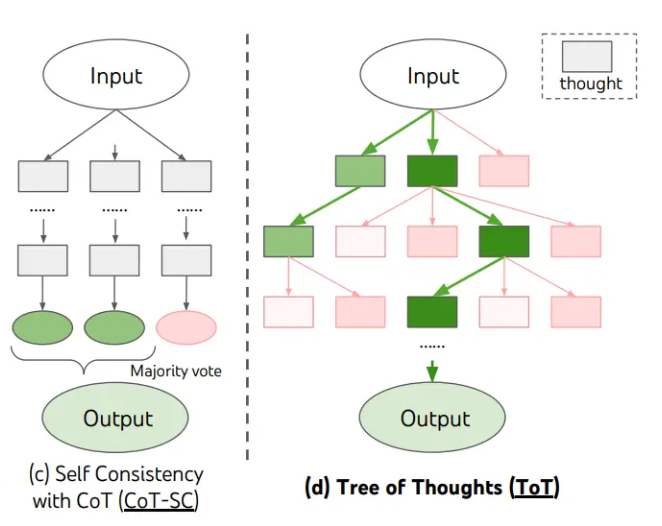
\includegraphics[width=0.8\textwidth,height=6.5cm,keepaspectratio]{Type.png}
        % Adjust the 0.8 value to resize
        % \caption{Comparison of Prompting Techniques:  Self Consistency with CoT (CoT-SC), and Tree of Thoughts (ToT).}
    \end{figure}
\end{frame}

\begin{frame}{Input-Output Prompting (IO)}

    \begin{itemize}
        \item \textcolor{black}{Direct relationship between input and output.}
        \item \textcolor{black}{Example:}
        \begin{itemize}
            \item \textbf{\textcolor{magenta}{Input:} \textcolor{black}{What is 2+2?}}
            \item \textbf{\textcolor{purple}{Output:} \textcolor{black}{4.}}
        \end{itemize}
    \end{itemize}

    \vspace{1cm} % Adds some vertical space between the list and the diagram

    \begin{center} % Centers the TikZ diagram
        \begin{tikzpicture}[node distance=6cm, auto]
            % Input Node
            \node[ellipse, draw, thick, align=center] (input) {Input};
            % Output Node
            \node[ellipse, draw, thick, align=center, right of=input] (output) {Output};
            % Arrow between Input and Output
            \draw[->, thick] (input) -- (output) node[midway, above] {Direct Response};
        \end{tikzpicture}
    \end{center}

\end{frame}

\begin{frame}{Game of 24 with the IO Prompt }
    \begin{tcolorbox}[
        colback=blue!10!white, 
        colframe=blue!70!black, 
        title=\textbf{\small Prompt}, 
        fonttitle=\bfseries\small, 
        coltitle=white, 
        boxrule=0.72mm, 
        sharp corners=southwest, 
        enhanced, 
        width=\textwidth-1.8cm, 
        enlarge left by=0.72cm
    ]
        
        \textbf{\small \textcolor{red}{Question}:}  
        Use numbers and basic arithmetic operations (\texttt{+}, \texttt{-}, \texttt{*}, \texttt{/}) to obtain 24.  
        Input: \( 4, 4, 6, 8 \)
        
        \vspace{0.54cm}
        
        \textbf{\small Solution:}  
        \[
        (8 - 6) \times (4 + 4) = 24
        \]

        \vspace{0.54cm}

        \textbf{\small Explanation:}
        \begin{itemize}
            \item \small Subtract \( 6 \) from \( 8 \):  \hspace{.45cm} 
            \textbf{\small 8 - 6 = 2}
            
            \item \small Add \( 4 \) and \( 4 \):  \hspace{1.35cm}\small 4 + 4 = 8
            \item \small Multiply the results from steps 1 and 2:  
            \[
            \small 2 \times 8 = 24
            \]
        \end{itemize}

    \end{tcolorbox}
\end{frame}
% \begin{frame}{Input-Output Prompting (IO)}

%     \begin{itemize}
%         \item \textcolor{green}{Merits:}
%         \begin{itemize}
%             \item[] \textbf{Straightforward}
%             \item[] \textbf{Minimal Instructions} 
%             \item[] \textbf{Ease of Understanding}
%             \item[] \textbf{Speed}
%         \end{itemize}\\
%         \vspace{0.5cm}
%         \item \textcolor{red}{Limitations:}
%         \begin{itemize}
%             \item[] \textbf{Lack of Complex Reasoning}
%             \item[] \textbf{Limited to Simple Queries} 
%             \item[] \textbf{No Contextual Awareness }
%             \item[] \textbf{Low Accuracy }
%             \item[] \textbf{Limited to One-Step Responses}
%         \end{itemize}
%     \end{itemize}
% \end{frame}

\begin{frame}{Input-Output Prompting (IO)}

    % Merits Box
    \begin{tcolorbox}[colback=green!10!white, colframe=green!70!black, title=\textbf{Merits}, fonttitle=\bfseries, coltitle=white, boxrule=0.8mm, sharp corners=southwest, enhanced, width=\textwidth-4cm, enlarge left by=1cm, drop shadow]
        \tiny % Resize the text inside the box further
        \begin{itemize}[label=\textcolor{green}{\scriptsize$\bullet$}, left=0pt, itemsep=0.2cm]
            \item \textbf{Straightforward}
            \item \textbf{Minimal Instructions}
            \item \textbf{Ease of Understanding}
            \item \textbf{Speed}
        \end{itemize}
    \end{tcolorbox}
    
    \vspace{0.2cm} % Adjust vertical space between boxes

    % Limitations Box
    \begin{tcolorbox}[colback=red!10!white, colframe=red!70!black, title=\textbf{Limitations}, fonttitle=\bfseries, coltitle=white, boxrule=0.8mm, sharp corners=southwest, enhanced, width=\textwidth-4cm, enlarge left by=1cm, drop shadow]
        \tiny % Resize the text inside the box further
        \begin{itemize}[label=\textcolor{red}{\scriptsize$\bullet$}, left=0pt, itemsep=0.2cm]
            \item \textbf{Lack of Complex Reasoning}
            \item \textbf{Limited to Simple Queries}
            \item \textbf{No Contextual Awareness}
            \item \textbf{Low Accuracy}
            \item \textbf{Limited to One-Step Responses}
        \end{itemize}
    \end{tcolorbox}
    
\end{frame}

\begin{frame}{Chain of Thought Prompting (CoT)}

    \begin{itemize}
        \item \textcolor{black}{Unlike I/O prompting, CoT guides the model to work through intermediate reasoning steps}
        \item \textcolor{black}{Encouraging Multi-Step Reasoning}
         \item \textcolor{black}{Achieving Efficiency without Finetuning}
        % \begin{itemize}
        %     \item \textbf{\textcolor{magenta}{Input:} \textcolor{black}{What is 2+2?}}
        %     \item \textbf{\textcolor{purple}{Output:} \textcolor{black}{4.}}
        % \end{itemize}
    \end{itemize}
\end{frame}
\begin{frame}{Chain of Thought Prompting (CoT)}
    \begin{figure}
        \centering
        
\includegraphics[width=0.8\textwidth,height=6.5cm,keepaspectratio]{COT.png}
        % Adjust the 0.8 value to resize
        % \caption{Comparison of Prompting Techniques:  Self Consistency with CoT (CoT-SC), and Tree of Thoughts (ToT).}
    \end{figure}
\end{frame}

\begin{frame}{Game of 24 with the COT Prompt}
    \begin{tcolorbox}[
        colback=blue!5!white, 
        colframe=blue!80!black, 
        title=\textbf{\scriptsize \textcolor{white}{Question and Solution}}, 
        fonttitle=\bfseries\scriptsize, 
        coltitle=white, 
        boxrule=0.75mm, 
        rounded corners, 
        width=\textwidth-1.5cm, 
        enlarge left by=0.75cm, 
        enhanced
    ]

        \textbf{\textcolor{red}{Question:}}  
        Use numbers and basic arithmetic operations (\texttt{+}, \texttt{-}, \texttt{*}, \texttt{/}) to obtain 24.  
        Each step, choose \textbf{two numbers} to perform an operation.  
        \textbf{Input:} \( 4, 4, 6, 8 \)

        \vspace{0.4cm}
        
        \textbf{\textcolor{green!50!black}{Solution:}}  
        \begin{itemize}
            \item \textbf{\textcolor{blue!70!black}{Start:}} \{4, 4, 6, 8\}
            \item Subtract \(8 - 6\): \textcolor{orange!70!black}{2} \hfill \textit{Remaining: \{4, 4, 2\}}
            \item Add \(4 + 4\): \textcolor{orange!70!black}{8} \hfill \textit{Remaining: \{8, 2\}}
            \item Multiply \(8 \times 2\): \textcolor{orange!70!black}{16} \hfill \textit{Remaining: \{16\}}
            \item Divide \(16 \div 8\): \textcolor{orange!70!black}{24} \hfill \textit{Final Result: \textbf{24}}
        \end{itemize}

        \vspace{0.4cm}
        \begin{center}
            \textbf{\textcolor{blue!60!black}{Result: \huge (8-6)x(4+4)\div 8}}
        \end{center}

    \end{tcolorbox}
\end{frame}

\begin{frame}{Chain of Thought Prompting (CoT)}

    % Merits Box
    \begin{tcolorbox}[colback=green!10!white, colframe=green!70!black, title=\textbf{Merits}, fonttitle=\bfseries, coltitle=white, boxrule=0.8mm, sharp corners=southwest, enhanced, width=\textwidth-3cm, enlarge left by=1cm, drop shadow]
        \small % Resize the text inside the box
        \begin{itemize}[label=\textcolor{green}{\scriptsize$\bullet$}, left=0pt, itemsep=0.2cm]
            \item \textbf{Mathematics and Arithmetic Problems solving}
            \item \textbf{Commonsense and Symbolic Reasoning}
            \item \textbf{Complex Decision-Making}
        \end{itemize}
    \end{tcolorbox}
    
    \vspace{0.4cm} % Adjust vertical space between boxes

    % Limitations Box
    \begin{tcolorbox}[colback=red!10!white, colframe=red!70!black, title=\textbf{Limitations}, fonttitle=\bfseries, coltitle=white, boxrule=0.8mm, sharp corners=southwest, enhanced, width=\textwidth-3cm, enlarge left by=1cm, drop shadow]
        \small % Resize the text inside the box
        \begin{itemize}[label=\textcolor{red}{\scriptsize$\bullet$}, left=0pt, itemsep=0.2cm]
            \item \textbf{Smaller models wrote illogical chains of thought}
            \item \textbf{CoT only yields performance gains when used with models of ∼100B parameters}
        \end{itemize}
    \end{tcolorbox}
    
\end{frame}

\begin{frame}{\textbf{Self-Consistency with Chain of Thought Prompting (CoT)}}
    
    \vspace{-1em}
    \begin{itemize}
        \item \textbf{\textcolor{myblue}{Step 1: Initiate with CoT/Few-shot Prompting}}  
        \begin{itemize}
            \item Use examples to demonstrate reasoning patterns.
            \item Start with a well-structured prompt that encourages step-by-step reasoning.
        \end{itemize}
        \vspace{0.5em}
        
        \item \textbf{\textcolor{mygreen}{Step 2: Generate Multiple Outputs}}
        \begin{itemize}
            \item Instead of one response, run the prompt multiple times.
            \item Obtain a variety of plausible answers.
        \end{itemize}
        \vspace{0.5em}
        
        \item \textbf{\textcolor{myorange}{Step 3: Select the Most Consistent Answer}}
        \begin{itemize}
            \item Aggregate all outputs from Step 2.
            \item Choose the most popular or consistent response as the final answer.
        \end{itemize}
    \end{itemize}
    
    % Add visual enhancements or callouts
  

\end{frame}

\begin{frame}{Self-Consistency with Chain of Thought Prompting (CoT)}
\begin{tikzpicture}[node distance=1.2cm and 2.5cm]

% Nodes
\node (prompt) [startstop] {CoT Prompt};
\node (response1) [response, right=of prompt, yshift=1.5cm] {LLM Response};
\node (response2) [response, right=of prompt, yshift=0.5cm] {LLM Response};
\node (response3) [response, right=of prompt, yshift=-0.5cm] {LLM Response};
\node (response4) [response, right=of prompt, yshift=-1.5cm] {LLM Response};
\node (voting) [process, right=of response2,xshift=0cm,yshift=-0.5cm] {Voting};
\node (answer) [startstop, right=of voting, xshift=0cm] {Answer};

% Arrows from prompt to responses
\draw [arrow] (prompt.east) -- ++(1cm,0) |- (response1.west);
\draw [arrow] (prompt.east) -- ++(1cm,0) |- (response2.west);
\draw [arrow] (prompt.east) -- ++(1cm,0) |- (response3.west);
\draw [arrow] (prompt.east) -- ++(1cm,0) |- (response4.west);

% Arrows from responses to voting
\draw [arrow] (response1.east) -- ++(1cm,0) |- (voting.west);
\draw [arrow] (response2.east) -- ++(1cm,0) |- (voting.west);
\draw [arrow] (response3.east) -- ++(1cm,0) |- (voting.west);
\draw [arrow] (response4.east) -- ++(1cm,0) |- (voting.west);

% Arrow from voting to answer
\draw [arrow] (voting.east) --++(1cm,0)|- (answer.west);

\end{tikzpicture}
\end{frame}

\begin{frame}{Game of 24 with the SC with COT Prompt}
    \begin{tcolorbox}[
        colback=blue!5!white, 
        colframe=blue!80!black, 
        title=\textbf{\textcolor{white}{Prompt }}, 
        fonttitle=\bfseries\scriptsize, 
        coltitle=white, 
        boxrule=0.75mm, 
        rounded corners, 
        width=\textwidth-1.5cm, 
        enlarge left by=0.75cm, 
        enhanced
    ]
        % Question Section
        \scriptsize
        \textbf{\textcolor{red}{Question:}}  
        \textit{Use numbers and basic arithmetic operations (+, -, *, /) to obtain 24. At each step, select two of the remaining numbers to calculate a new number. Repeat for various combinations and select the best solution.}  
        \hfill \textbf{Input:} \{4, 4, 6, 8\}

        \vspace{0.3cm}
        
        % Solution Section
        \textbf{\textcolor{green!50!black}{Optimized Solution:}}  
        \begin{itemize}
            \item \textbf{\textcolor{blue!70!black}{Step 1:}} Subtract \(6- 4 = 2\) \hfill \textit{Remaining: \{4, 8, 2\}}
            \item \textbf{\textcolor{blue!70!black}{Step 2:}} Add \(4 + 8 = 12\) \hfill \textit{Remaining: \{12, 2\}}
            \item \textbf{\textcolor{blue!70!black}{Step 3:}} Multiply \(12 \times 2 = 24\) 
           \hfill \textit{Final Result: \textbf{24}}
        \end{itemize}
        
        \vspace{0.3cm}
        \begin{center}
            \tcbset{colback=green!10!white, colframe=green!60!black, boxrule=1mm, width=\textwidth-2cm, rounded corners}
            \begin{tcolorbox}[sharp corners=south, coltitle=black]
                \textbf{\small Final Answer:} \textbf{\huge (6-4)x(4+8)}
            \end{tcolorbox}
        \end{center}

    \end{tcolorbox}
\end{frame}

\begin{frame}{Self-Consistency with Chain of Thought Prompting (CoT)}

    % Merits Box
    \begin{tcolorbox}[colback=green!10!white, colframe=green!70!black, title=\textbf{Merits}, fonttitle=\bfseries, coltitle=white, boxrule=0.8mm, sharp corners=southwest, enhanced, width=\textwidth-3cm, enlarge left by=1cm, drop shadow]
        \small % Resize the text inside the box
        \begin{itemize}[label=\textcolor{green}{\scriptsize$\bullet$}, left=0pt, itemsep=0.2cm]
            \item \textbf{Improved Accuracy and Reasoning}
            \item \textbf{Helps with Complex Problem Solving}
            \item \textbf{Improved Explanations}
        \end{itemize}
    \end{tcolorbox}
    
    \vspace{0.4cm} % Adjust vertical space between boxes

    % Limitations Box
    \begin{tcolorbox}[colback=red!10!white, colframe=red!70!black, title=\textbf{Limitations}, fonttitle=\bfseries, coltitle=white, boxrule=0.8mm, sharp corners=southwest, enhanced, width=\textwidth-3cm, enlarge left by=1cm, drop shadow]
        \small % Resize the text inside the box
        \begin{itemize}[label=\textcolor{red}{\scriptsize$\bullet$}, left=0pt, itemsep=0.2cm]
            \item \textbf{Difficulty in Scaling}
            \item \textbf{Vulnerable to Misleading Intermediate Steps}
            \item \textbf{Potential for Ambiguity in Steps}
            % \item \textbf{Vulnerable to Misleading Intermediate Steps}
        \end{itemize}
    \end{tcolorbox}
    
\end{frame}
\begin{frame}{Next}
    \begin{figure}
        \centering
        
\includegraphics[width=0.8\textwidth,height=6.5cm,keepaspectratio]{wh.png}
        % Adjust the 0.8 value to resize
        % \caption{Comparison of Prompting Techniques:  Self Consistency with CoT (CoT-SC), and Tree of Thoughts (ToT).}
    \end{figure}
\end{frame}

\section{How Human Thinks!}

\begin{frame}{Ways of Thinking}
Two ways of thinking:
    \begin{itemize}
        \item Common people with a random thought process.
            \only<1>{%
            \begin{tikzpicture}[remember picture, overlay]
                \draw[->, thick] (0.2,0.1) -- (3,0.1) node[midway, above] {};
                \node at (4, 0) {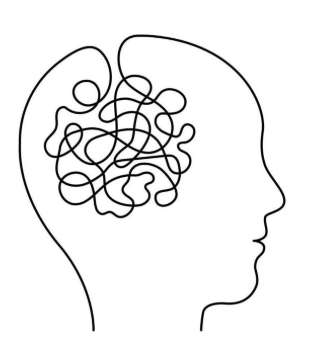
\includegraphics[width=1.5cm]{ImagesAlif/Random Thought.png}}; % Replace with your image file
            \end{tikzpicture}}
        \only<2>{    
        \item Logical and well-thought process of a Mathematician.
            %
            \begin{tikzpicture}[remember picture, overlay]
                \draw[->, thick] (0.2,0.1) -- (3,0.1) node[midway, above] {};
                \node at (4, 0) {
\includegraphics[width=1.5cm]{ImagesAlif/Structured Thinking.png}}; % Replace with your image file
            \end{tikzpicture}}
    \end{itemize}
\end{frame}



\begin{frame}{Random Thinking And Its Limitations}
    \begin{itemize}
        \item Many people may approach the "Game of 24" with random operations. For Example:
    \end{itemize}

    \begin{block}{Random Approach}
    \begin{itemize}
\centering
        \item Chose 14, 3 and multiply them
        
        
        \begin{tikzpicture}[node distance=1.5cm and 2.5cm, >=latex]
            % Nodes for numbers
            \node (num1) [draw, circle, fill=blue!10, align=center] at (0, 3) {14,3};
            \node (num2) [draw, circle, fill=green!10, align=center] at (3, 3) {42};
            \draw[->, thick] (num1) -- node[midway, above] {*} (num2);
        \end{tikzpicture}
        \pause
        \item Now divide this 42 by 7
        
        
        \begin{tikzpicture}[node distance=1.5cm and 2.5cm, >=latex]
            \node (num1) [draw, circle, fill=blue!10, align=center] at (0, -3) {42,7};
            \node (num2) [draw, circle, fill=green!10, align=center] at (3, -3) {6};
            \draw[->, thick] (num1) -- node[midway, above] {/} (num2);
        \end{tikzpicture}
        \pause
        \item Now again multiply this 6 with 3
        
        
        \begin{tikzpicture}[node distance=1.5cm and 2.5cm, >=latex]
            \node (num1) [draw, circle, fill=blue!10, align=center] at (4, -3) {6,3};
            \node (num2) [draw, circle, fill=green!10, align=center] at (7, -3) {18 \\ OOOPS!};
            \draw[->, thick] (num1) -- node[midway, above] {*} (num2);
        \end{tikzpicture}
    \end{itemize}
    \end{block}
\end{frame}

\begin{frame}{Random Thinking and Its Limitations}
From the previous slide, we see that a random approach to problem-solving is not very effective. Therefore, we propose:
    \begin{itemize}
    
         \item While random guessing might occasionally work for humans, it is inefficient and unreliable for machines.
         
         \only<1>{%
            \begin{tikzpicture}[remember picture, overlay]
                \draw[->, thick] (5,0.1) -- (5,-.5) node[midway, above] {};
                \node at (5, -1.5) {
\includegraphics[width=1.5cm]{ImagesAlif/Dont.jpg}}; % Replace with your image file
            \end{tikzpicture}}
            \only<2>{
         \item Instead, we will adopt the structured and systematic thought process of a mathematician.}
    \end{itemize}
\end{frame}


\begin{frame}{How Mathematicians Solve Problems}
How a mathematician will solve "Game of 24"! What are the differences?\\
\begin{tikzpicture}

\only<1>{\node at (-5,3.5)
\includegraphics[width =3.5cm]{ImagesAlif/Thinking.jpg}}
    
\end{tikzpicture}
\pause

A mathematician solves problems systematically:
    \begin{itemize}
         \item First He will try to sort the inputs.
         \begin{tikzpicture}

\only<2>{\node at (2,1.5)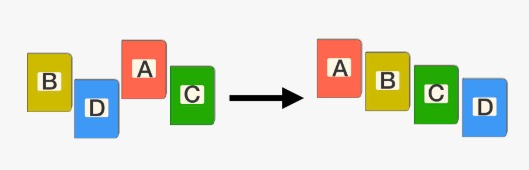
\includegraphics[width =3.5cm]{ImagesAlif/Sorting.jpg}}
    
\end{tikzpicture}
\pause
        
            \item Evaluate whether it is even possible to reach 24.
                    \begin{tikzpicture}

\only<3>{\node at (4,3)
\includegraphics[width =3.5cm]{ImagesAlif/Possible.jpg}}
    
\end{tikzpicture}
\pause
            \item Explore logical paths using operations and combinations.
                                \begin{tikzpicture}

\only<4>{\node at (5.5,2.5)
\includegraphics[width =4cm]{ImagesAlif/Exploring.jpg}}
    
\end{tikzpicture}
\pause
            \item Refine results to find the solution.
    \end{itemize}
\end{frame}

\begin{frame}{Step 1: Sorting and Initial Evaluation}
    \begin{itemize}
        \item Sort the inputs: \( 3, 5, 7, 14 \).
        \pause
        \item Check if any number is greater than 24 (None here).
        \pause
        \item Multiply all numbers: \( 3 \times 5 \times 7 \times 14 = 1470 \).
        \pause
        \item Since \( 1470 > 24 \), a solution is possible.
    \end{itemize}
    \vspace{0.5cm}
    
\end{frame}
\begin{frame}{Step 2: Finding the Largest Number And Possible Solution}
    \begin{itemize}
        \item The largest number is \( 14 \).
        \pause
        \item Check if the remaining numbers (\( 3, 5, 7 \)) can form \( 10 \): Not possible.
        \pause
        \item Move to the next step by exploring pairs.
    \end{itemize}
    \vspace{0.5cm}
   
\end{frame}

\begin{frame}{Step 3: Pairing and Operations}
    Explore all pairs:
    \[
    \begin{aligned}
        (3,5) &\quad \rightarrow \quad 3+5=8, \ 3 \times 5=15, \ 3-5=-2, \ 3/5=0.6 \\
        (5,7) &\quad \rightarrow \quad 5+7=12, \ 5 \times 7=35, \ \ldots \\
        \ldots &\quad \text{(Other pairs similarly explored)} \\
    \end{aligned}
    \]
    \pause
    \vspace{0.5cm}
    Highlight: \( 5 \times 7 = 35 \), which is a promising result.\\
    \pause
    The remaining digits are 3 and 14 .
\end{frame}
\begin{frame}{Step 4: Finding the Missing Subtractor}
    \begin{itemize}
        \item From \( 35 \), He needs to subtract \( 11 \) to reach \( 24 \).
        \pause
        \item He checks the remaining numbers: \( 14 - 3 = 11 \), the desired subtractor.
        
    \end{itemize}
    \[
    35 - 11 = 24
    \]
    \centering
    \vspace{-1cm}
    \begin{tikzpicture}
        
    
     \filldraw[rounded corners=3pt, fill=red!20, draw=blue!50, thick] (2.5,0) rectangle (12.5,0.5);
    \node[align=center, text width=7cm, font=\small] at (8,0.2) {PROBLEM SOLVED !!!!!!!!!!!!!!!!};
    \end{tikzpicture}
    \vspace{0.5cm}
    
   
\end{frame}

\begin{frame}{Bringing All Steps Together}
    
    
  \begin{tikzpicture}
    \draw[->, thick] (-3.5,4.75) -- (-2,4.75) node[midway, above] {Start};
    \pause
    \filldraw[rounded corners=3pt, fill=blue!20, draw=blue!50, thick] (-2,4) rectangle (-0.5,5.5);
   \node[align=center, text width=1.4cm, font=\small] at (-1.25,4.75) {Digits: 14,5,7,3};
   \draw[->, thick] (-0.5,4.75) -- (0.5,4.75);
   \pause
   \filldraw[rounded corners=3pt, fill=blue!20, draw=blue!50, thick] (0.5,4) rectangle (2,5.5);
   \node[align=center, text width=1.4cm, font=\small] at (1.25,4.75) {Sort them: 3,5,7,14};
   \filldraw[rounded corners=3pt, fill=blue!20, draw=blue!50, thick] (0.5,4) rectangle (2,5.5);
   \node[align=center, text width=1.4cm, font=\small] at (1.25,4.75) {Sort them: 3,5,7,14};
   \draw[->, thick] (2,4.75) -- (3,4.75);
   \pause
    \filldraw[rounded corners=3pt, fill=blue!20, draw=blue!50, thick] (3,4) rectangle (4.5,5.5);
    \node[align=center, text width=1.4cm, font=\tiny] at (3.75,4.75) {All digits $<$ 24. Largest: 14, others don't sum to 10.};
     \draw[->, thick] (4.5,4.75) -- (5.5,4.75);
     \pause
    \filldraw[rounded corners=3pt, fill=blue!20, draw=blue!50, thick] (5.5,4) rectangle (7,5.5);
    \node[align=center, text width=1.4cm, font=\tiny] at (6.25,4.75) {Pair digits and compute useful results.};
    \draw[->, thick] (7,4.75) -- (8,4.75);
    \pause
    \filldraw[rounded corners=3pt, fill=blue!20, draw=blue!50, thick] (8,4) rectangle (9.5,5.5);
    \node[align=center, text width=1.4cm, font=\tiny] at (8.75,4.75) {Found 35 from $5*7$ a promising result.};
    \draw[->, thick] (8.75,4) -- (8.75,3);
    \pause
     \filldraw[rounded corners=3pt, fill=blue!20, draw=blue!50, thick] (8,3) rectangle (9.5,1.5);
    \node[align=center, text width=1.4cm, font=\tiny] at (8.75,2.25) {Can he make 11 from remaining two digits!};
    \draw[->, thick] (8,2.25) -- (7,2.25);
    \pause
    \filldraw[rounded corners=3pt, fill=blue!20, draw=blue!50, thick] (5.5,3) rectangle (7,1.5);
    \node[align=center, text width=1.4cm, font=\tiny] at (6.25,2.25) {Can he make $11$ using the remaining two digits?};
    \draw[->, thick] (5.5,2.25) -- (4.5,2.25);
    \pause
    \filldraw[rounded corners=3pt, fill=blue!20, draw=blue!50, thick] (3,3) rectangle (4.5,1.5);
    \node[align=center, text width=1.4cm, font=\tiny] at (3.75,2.25) {Yes! Subtract $14$ and $3$ to get $11$. Subtract $11$ from $35$. Final Result: $24$.};
    \pause
    \node[anchor=west] at (-1,2.25) {
\includegraphics[width=3cm]{ImagesAlif/Eureka.jpg}};
    \filldraw[rounded corners=3pt, fill=red!20, draw=blue!50, thick] (-0.5,0) rectangle (8.5,0.5);
    \node[align=center, text width=7cm, font=\small] at (4,0.2) {Solution: $5*7-14+3=24$};



\end{tikzpicture}
\end{frame}

\begin{frame}{Advantages of Structured Thinking in Problem Solving}
    \begin{itemize}
        \item Structured reasoning eliminates random guesses and focuses on promising paths.
        \pause
        \item Logical exploration ensures efficiency and clarity in problem-solving.
        \pause
        \item This approach is not just for puzzles but applies to many areas of reasoning.
    \end{itemize}
    \vspace{0.5cm}
  
\end{frame}

\section{Modeling Human Problem-Solving in Language Models}
\begin{frame}{Modeling Human Problem-Solving in Language Models}
\begin{block}{Steps To solve the problem using AI tools using ToT prompting}

\begin{itemize}
\centering
    \item Problem Decomposition.
    
    \pause
    \item Thought Generation.
    \pause
    \item State Evaluation.
    \pause
    \item  Decision Making.
\end{itemize}
    
\end{block}
\end{frame}
\begin{frame}{Step 1: Problem Decomposition}
    Language Models systematically break the problem into smaller parts:
    \begin{itemize}
        \item \textbf{Input Analysis:} Identify the components:
        \begin{itemize}
            \item Numbers: \(3, 5, 7, 14\)
            \item Target: \(24\)
        \end{itemize}
        \pause
        \item In this step pairs of inputs are made.
        \item \textbf{Pair the Inputs:}
        \begin{center}
            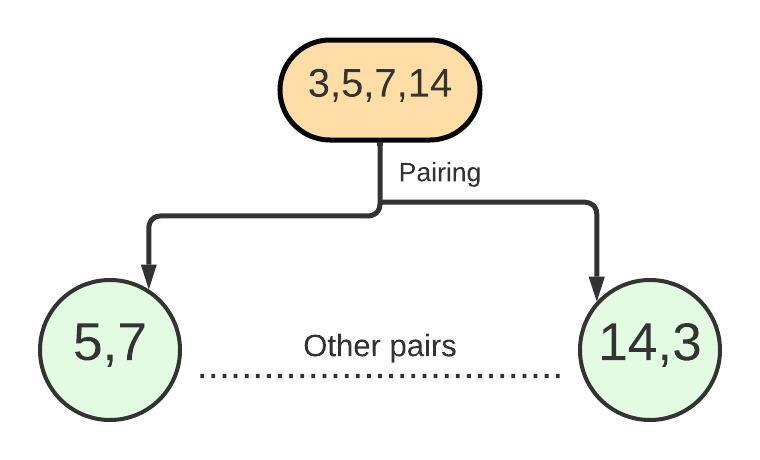
\includegraphics[width=6cm]{ImagesAlif/Org chart.jpeg}
        \end{center}
    \end{itemize}
\end{frame}
\begin{frame}{Step 2: Thought Generation}
    Language Models explore multiple paths to generate solutions:
    \begin{itemize}
        \item \textbf{Objective:} Systematically compute results from the pairs generated in the decomposition step and apply operations to approach the target \(24\).
        \pause
        \item From the decomposition step, pairs such as \((5, 7)\) and \((14, 3)\) are identified.
        \pause
        \item Different arithmetic operations are performed on these pairs to generate intermediate values. 
        \item For example:
        \begin{center}
            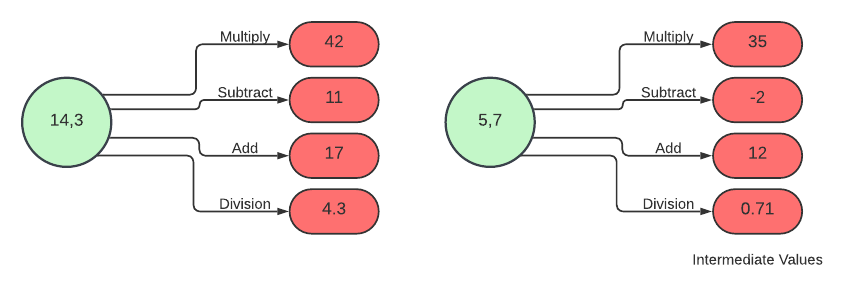
\includegraphics[width=12cm]{ImagesAlif/Org chart.png}
        \end{center}
    \end{itemize}
\end{frame}

% \begin{frame}{Step 3: State Evaluation}
%     Language Models refine their approach at each step by evaluating intermediate values to determine their potential to reach the target. Promising paths are identified and explored further, while unproductive paths are discarded.
%     \begin{itemize}
%         \item \textbf{Objective:} Evaluate intermediate steps to ensure progress toward the target \(24\).
%         \pause
%         \item \textbf{Evaluation Criteria:}  
%         Each step is assessed based on:
%         \begin{itemize}
%             \item \textbf{Proximity to the Target:} Does the result move closer to \(24\)?
%             \item \textbf{Operation Validity:} Are the mathematical operations valid (e.g., no division by zero)?
%             \item \textbf{Feasibility:} Does the intermediate result allow for a viable path to the solution?
%             \item If progress toward the target is possible, calculations continue; otherwise, the path is terminated.
%         \end{itemize}
%         \pause
%     \end{itemize}
% \end{frame}

% \begin{frame}{Step 3: State Evaluation (Visualized)}
% \begin{center}
%     \only<1>{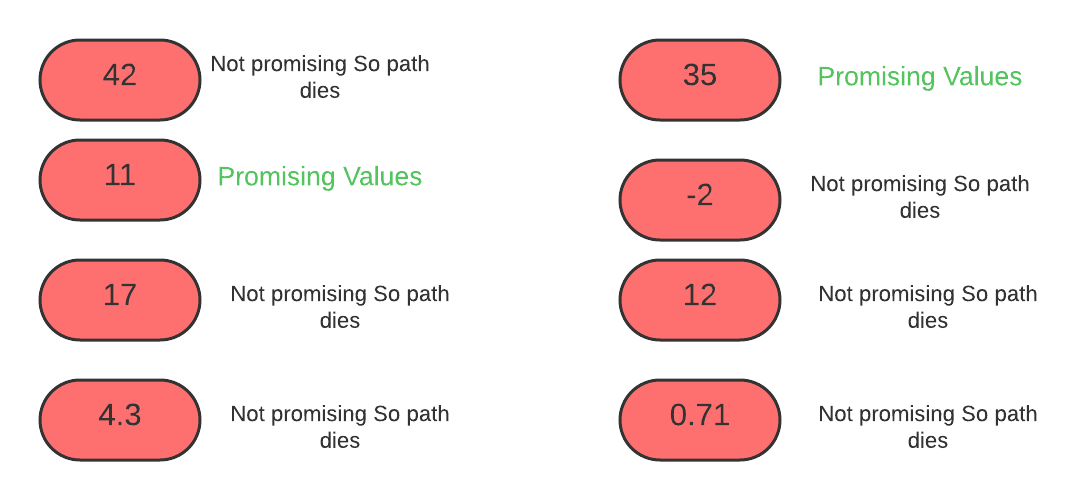
\includegraphics[width=12cm]{ImagesAlif/Org chart (1).png}}
%     \only<2>{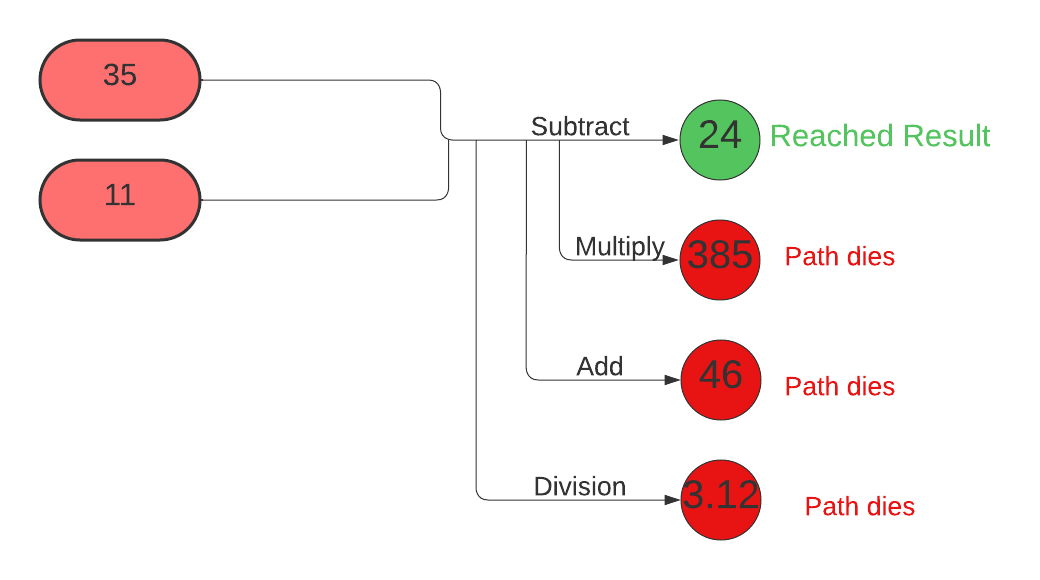
\includegraphics[width=12cm]{ImagesAlif/Org chart (2).png}}
% \end{center}
% \end{frame}


% \begin{frame}{All three steps Combined }
%     \begin{center}
%         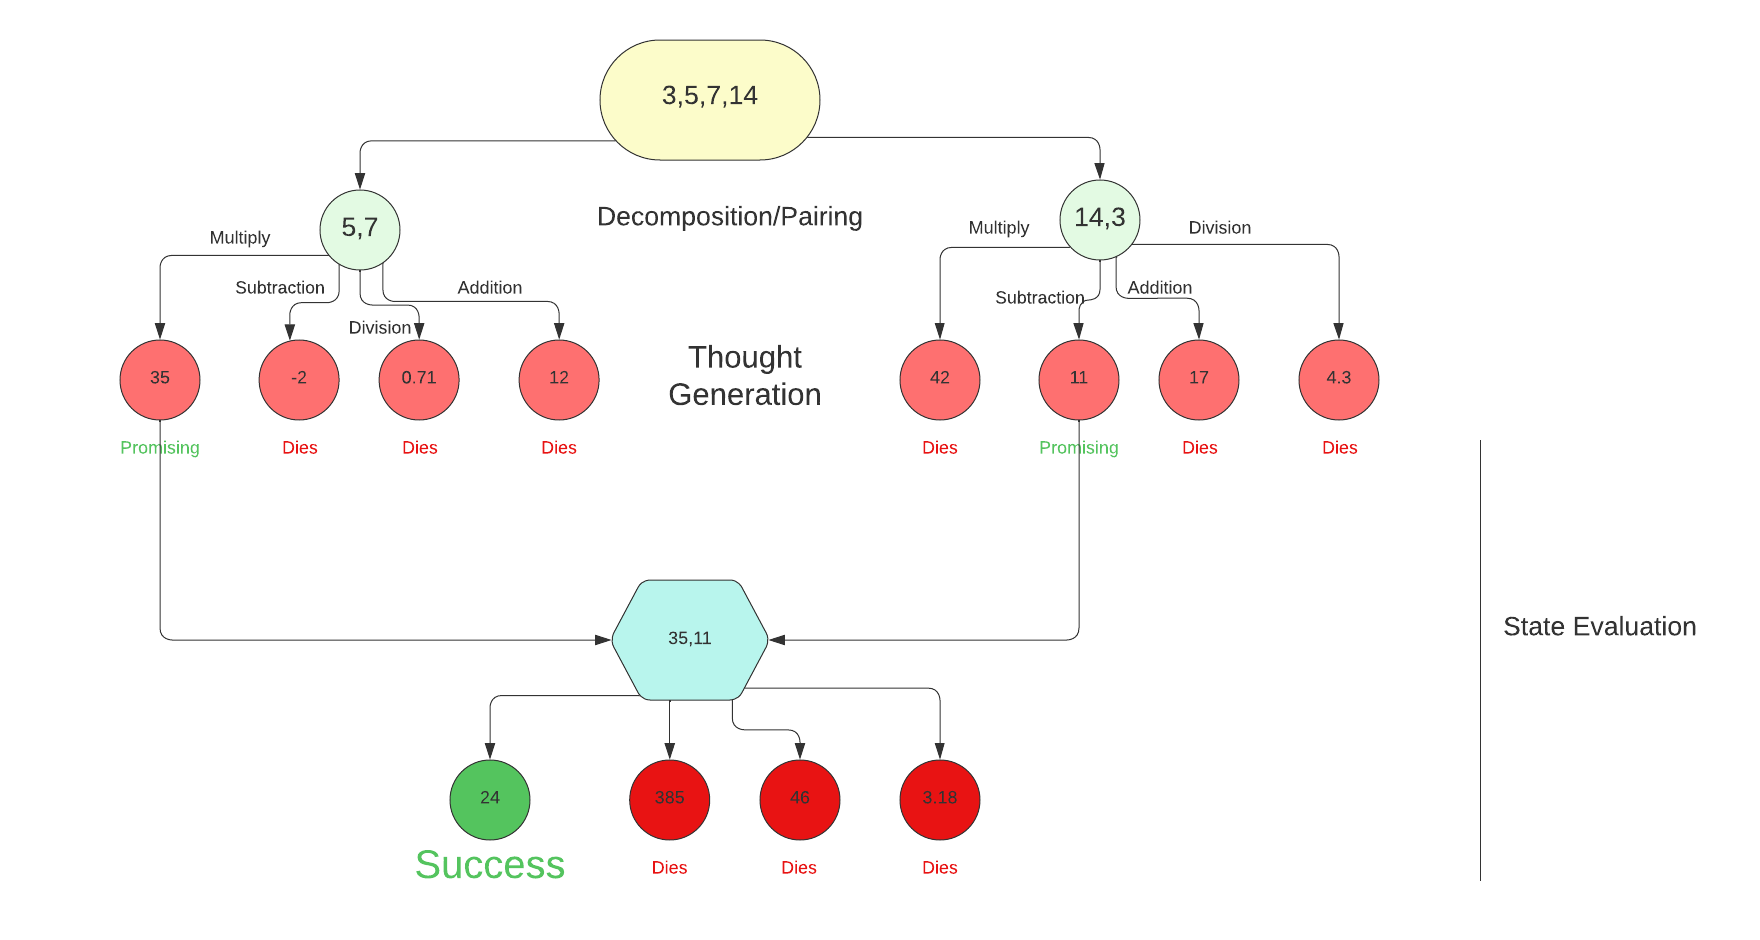
\includegraphics[width=14cm]{ImagesAlif/Org chart (3).png}
%     \end{center}
% \end{frame}








%hamim
\section{Example}

\begin{frame}{Game of 24 Prompt}
\textbf{Conceptual Stages or Processes:}
\vspace{.3cm}
\begin{itemize}
    \item \textbf{Propose Prompt}
    \item \textbf{Value Prompt}
    
    
\end{itemize}
\end{frame}


\begin{frame}{Game of 24 Prompt}
    \begin{tcolorbox}[
        colback=gray!5!white, 
        colframe=black!50!white, 
        title=\textbf{\small Propose Prompt}, 
        fonttitle=\bfseries\small, 
        coltitle=white, 
        boxrule=0.72mm, 
        sharp corners=southwest, 
        enhanced, 
        width=\textwidth-1.8cm, 
        enlarge left by=0.72cm
    ]
        
        \textbf{\small \textcolor{red}{User}:}  
        Game of 24 is a mathematical reasoning challenge, where the goal is to use 4 numbers and basic
arithmetic operations (+,-,*,/) to obtain 24.
input: 3,5,7,14
give me all the possible next step that will left me with 3 input value \\
\\
\textbf{\textcolor{orange}{Assistant}:}To determine all possible next steps in the "Game of 24" for the input numbers 3,5,7,14, we combine any two numbers using the basic arithmetic operations (+,−,∗,/), provided division results in an integer. This reduces the number of inputs from 4 to 3.\\
\textbf{Steps:}
\begin{itemize}
    \item Pair any two numbers (e.g., \(3\) and \(5\)).
    \item Apply each valid operation to create a new number.
    \item Replace the pair with the result, leaving three numbers.
\end{itemize}
    \end{tcolorbox}
\end{frame}

\begin{frame}{Game of 24 Prompt}
\centering
\begin{tcolorbox}[
    colback=gray!5!white, colframe=black!50!white,
    title=Propose Prompt Continue,
    fonttitle=\bfseries, rounded corners, boxrule=1mm,
    width=\textwidth
]


\textbf{Combinations and Results}\\
\\
\textbf{1. Pair \(3\) and \(5\):}

\begin{itemize}
    \item \(3 + 5 = 8 \quad \rightarrow \quad \text{Remaining: } 8, 7, 14\)
    \item \(3 - 5 = -2 \quad \rightarrow \quad \text{Remaining: } -2, 7, 14\)
    \item \(5 - 3 = 2 \quad \rightarrow \quad \text{Remaining: } 2, 7, 14\)
    \item \(3 \times 5 = 15 \quad \rightarrow \quad \text{Remaining: } 15, 7, 14\)
\end{itemize}

\end{tcolorbox}

\end{frame}


% treee
\begin{frame}{Game of 24}
\centering
    \begin{left}
    \begin{tikzpicture}[ 
    box/.style={draw, rounded corners, minimum width=0.2cm, minimum height=.4cm,align=center},
    rootbox/.style={draw, rounded corners, minimum width=.7cm, minimum height=.3cm,text width=1cm,align=center},
    arrow/.style={->, thick, >=latex, draw=gray!60},
    level 1/.style={sibling distance=2.5cm,level distance=2.5cm},
    level 2/.style={sibling distance=2cm},
    level 3/.style={sibling distance=2cm},
    level 4/.style={sibling distance=2cm}
]
    % Root node
    \node[box, fill=yellow!10] (root) {
    \\
    input:\\ 3, 5 , 7, 14

    }

     % % Level 1
     %    child { node[box, fill=orange!20] {3+5=8\\ →8,7,14} 
     %        % % Level 2 for 1a
     %        % child { node[box, fill=red!20] {Level 2a}
     %        %     % Level 3 for 2a
     %        %     child { node[box, fill=blue!20] {Level 3a}
     %        %         % Level 4 for 3a
     %        %         child { node[box, fill=green!20] {Level 4a} }
     %        %         child { node[box, fill=green!20] {Level 4b} }
     %        %     }
     %        %     child { node[box, fill=blue!20] {Level 3b} }
     %        % }
     %        % child { node[box, fill=red!20] {Level 2b} }
     %    }
     %    child { node[box, fill=orange!20] {5×7=35\\→35,3,14} 
     %        % % Level 2 for 1a
     %        child { node[box, fill=red!20] {35 - 3=32\\ →32,14}
     %            % Level 3 for 2a
     %            % child { node[box, fill=blue!20] {Level 3a}
     %            %     % Level 4 for 3a
     %            %     child { node[box, fill=green!20] {Level 4a} }
     %            %     child { node[box, fill=green!20] {Level 4b} }
     %            % }
     %            % child { node[box, fill=blue!20] {Level 3b} }
     %        }
     %        child { node[box, fill=red!20] {35 - 14=21\\ →21,3} }
     %        child { node[box, fill=red!20] {3-14=-11 \\→-11,35} }
     %    }
     %    child { node[box, fill=orange!20] {7 - 3=4 \\→ 4,5,14} 
     %        % % Level 2 for 1a
     %        % child { node[box, fill=red!20] {Level 2a}
     %        %     % Level 3 for 2a
     %        %     child { node[box, fill=blue!20] {Level 3a}
     %        %         % Level 4 for 3a
     %        %         child { node[box, fill=green!20] {Level 4a} }
     %        %         child { node[box, fill=green!20] {Level 4b} }
     %        %     }
     %        %     child { node[box, fill=blue!20] {Level 3b} }
     %        % }
     %        % child { node[box, fill=red!20] {Level 2b} }
     %    }
     %    child { node[box, fill=orange!20] {14/3=4.666 \\(invalid)} 
     %        % % Level 2 for 1a
     %        % child { node[box, fill=red!20] {Level 2a}
     %        %     % Level 3 for 2a
     %        %     child { node[box, fill=blue!20] {Level 3a}
     %        %         % Level 4 for 3a
     %        %         child { node[box, fill=green!20] {Level 4a} }
     %        %         child { node[box, fill=green!20] {Level 4b} }
     %        %     }
     %        %     child { node[box, fill=blue!20] {Level 3b} }
     %        % }
     %        % child { node[box, fill=red!20] {Level 2b} }
     %    }
     %    child { node[box, fill=orange!20] {14/7=2 \\→2,3,5} 
     %        % % Level 2 for 1a
     %        child { node[box, fill=red!20] {2 * 3= 6\\ →6,5}
     %            % Level 3 for 2a
     %            % child { node[box, fill=blue!20] {Level 3a}
     %            %     % Level 4 for 3a
     %            %     child { node[box, fill=green!20] {Level 4a} }
     %            %     child { node[box, fill=green!20] {Level 4b} }
     %            % }
     %            % child { node[box, fill=blue!20] {Level 3b} }
     %        }
     %        child { node[box, fill=red!20] {3+5=8\\→8,2} }
     %    }
     %    child { node[box, fill=orange!20] {5×14=70\\ → 70,3,7} 
     %        % % Level 2 for 1b
     %        child { node[box, fill=red!20] {70/7=10\\→10,3}
     %            % % Level 3 for 2c
     %            % child { node[box, fill=blue!20] {Level 3c}
     %            %     % Level 4 for 3c
     %            %     child { node[box, fill=green!20] {Level 4c} }
     %            %     child { node[box, fill=green!20] {Level 4d} }
     %            % }
     %        }
     %    };

       

    \end{tikzpicture}
    \end{left}
\end{frame}

\begin{frame}{Game of 24}
\centering
    \begin{left}
    \begin{tikzpicture}[ 
    box/.style={draw, rounded corners, minimum width=0.2cm, minimum height=.4cm,align=center},
    rootbox/.style={draw, rounded corners, minimum width=.7cm, minimum height=.3cm,text width=1cm,align=center},
    arrow/.style={->, thick, >=latex, draw=gray!60},
    level 1/.style={sibling distance=2.5cm,level distance=2.5cm},
    level 2/.style={sibling distance=2cm},
    level 3/.style={sibling distance=2cm},
    level 4/.style={sibling distance=2cm}
]
    % Root node
    \node[box, fill=yellow!10] (root) {
    \\
    input:\\ 3, 5 , 7, 14

    }

     % Level 1
        child { node[box, fill=orange!20] {3+5=8\\ →8,7,14} 
            % % Level 2 for 1a
            % child { node[box, fill=red!20] {Level 2a}
            %     % Level 3 for 2a
            %     child { node[box, fill=blue!20] {Level 3a}
            %         % Level 4 for 3a
            %         child { node[box, fill=green!20] {Level 4a} }
            %         child { node[box, fill=green!20] {Level 4b} }
            %     }
            %     child { node[box, fill=blue!20] {Level 3b} }
            % }
            % child { node[box, fill=red!20] {Level 2b} }
        }
        % child { node[box, fill=orange!20] {5×7=35\\→35,3,14} 
        %     % % Level 2 for 1a
        %     child { node[box, fill=red!20] {35 - 3=32\\ →32,14}
        %         % Level 3 for 2a
        %         % child { node[box, fill=blue!20] {Level 3a}
        %         %     % Level 4 for 3a
        %         %     child { node[box, fill=green!20] {Level 4a} }
        %         %     child { node[box, fill=green!20] {Level 4b} }
        %         % }
        %         % child { node[box, fill=blue!20] {Level 3b} }
        %     }
        %     child { node[box, fill=red!20] {35 - 14=21\\ →21,3} }
        %     child { node[box, fill=red!20] {3-14=-11 \\→-11,35} }
        % }
        % child { node[box, fill=orange!20] {7 - 3=4 \\→ 4,5,14} 
        %     % % Level 2 for 1a
        %     % child { node[box, fill=red!20] {Level 2a}
        %     %     % Level 3 for 2a
        %     %     child { node[box, fill=blue!20] {Level 3a}
        %     %         % Level 4 for 3a
        %     %         child { node[box, fill=green!20] {Level 4a} }
        %     %         child { node[box, fill=green!20] {Level 4b} }
        %     %     }
        %     %     child { node[box, fill=blue!20] {Level 3b} }
        %     % }
        %     % child { node[box, fill=red!20] {Level 2b} }
        % }
        % child { node[box, fill=orange!20] {14/3=4.666 \\(invalid)} 
        %     % % Level 2 for 1a
        %     % child { node[box, fill=red!20] {Level 2a}
        %     %     % Level 3 for 2a
        %     %     child { node[box, fill=blue!20] {Level 3a}
        %     %         % Level 4 for 3a
        %     %         child { node[box, fill=green!20] {Level 4a} }
        %     %         child { node[box, fill=green!20] {Level 4b} }
        %     %     }
        %     %     child { node[box, fill=blue!20] {Level 3b} }
        %     % }
        %     % child { node[box, fill=red!20] {Level 2b} }
        % }
        % child { node[box, fill=orange!20] {14/7=2 \\→2,3,5} 
        %     % % Level 2 for 1a
        %     child { node[box, fill=red!20] {2 * 3= 6\\ →6,5}
        %         % Level 3 for 2a
        %         % child { node[box, fill=blue!20] {Level 3a}
        %         %     % Level 4 for 3a
        %         %     child { node[box, fill=green!20] {Level 4a} }
        %         %     child { node[box, fill=green!20] {Level 4b} }
        %         % }
        %         % child { node[box, fill=blue!20] {Level 3b} }
        %     }
        %     child { node[box, fill=red!20] {3+5=8\\→8,2} }
        % }
        % child { node[box, fill=orange!20] {5×14=70\\ → 70,3,7} 
        %     % % Level 2 for 1b
        %     child { node[box, fill=red!20] {70/7=10\\→10,3}
        %         % % Level 3 for 2c
        %         % child { node[box, fill=blue!20] {Level 3c}
        %         %     % Level 4 for 3c
        %         %     child { node[box, fill=green!20] {Level 4c} }
        %         %     child { node[box, fill=green!20] {Level 4d} }
        %         % }
        %     }
        % };

       

    \end{tikzpicture}
    \end{left}
\end{frame}

\begin{frame}{Game of 24}
\centering
    \begin{left}
    \begin{tikzpicture}[ 
    box/.style={draw, rounded corners, minimum width=0.2cm, minimum height=.4cm,align=center},
    rootbox/.style={draw, rounded corners, minimum width=.7cm, minimum height=.3cm,text width=1cm,align=center},
    arrow/.style={->, thick, >=latex, draw=gray!60},
    level 1/.style={sibling distance=2.5cm,level distance=2.5cm},
    level 2/.style={sibling distance=2cm},
    level 3/.style={sibling distance=2cm},
    level 4/.style={sibling distance=2cm}
]
    % Root node
    \node[box, fill=yellow!10] (root) {
    \\
    input:\\ 3, 5 , 7, 14

    }

     % Level 1
        child { node[box, fill=orange!20] {3+5=8\\ →8,7,14} 
            % % Level 2 for 1a
            % child { node[box, fill=red!20] {Level 2a}
            %     % Level 3 for 2a
            %     child { node[box, fill=blue!20] {Level 3a}
            %         % Level 4 for 3a
            %         child { node[box, fill=green!20] {Level 4a} }
            %         child { node[box, fill=green!20] {Level 4b} }
            %     }
            %     child { node[box, fill=blue!20] {Level 3b} }
            % }
            % child { node[box, fill=red!20] {Level 2b} }
        }
        child { node[box, fill=orange!20] {5×7=35\\→35,3,14} 
            % % Level 2 for 1a
            % child { node[box, fill=red!20] {35 - 3=32\\ →32,14}
            %     % Level 3 for 2a
            %     % child { node[box, fill=blue!20] {Level 3a}
            %     %     % Level 4 for 3a
            %     %     child { node[box, fill=green!20] {Level 4a} }
            %     %     child { node[box, fill=green!20] {Level 4b} }
            %     % }
            %     % child { node[box, fill=blue!20] {Level 3b} }
            % }
            % child { node[box, fill=red!20] {35 - 14=21\\ →21,3} }
            % child { node[box, fill=red!20] {3-14=-11 \\→-11,35} }
        }
        % child { node[box, fill=orange!20] {7 - 3=4 \\→ 4,5,14} 
        %     % % Level 2 for 1a
        %     % child { node[box, fill=red!20] {Level 2a}
        %     %     % Level 3 for 2a
        %     %     child { node[box, fill=blue!20] {Level 3a}
        %     %         % Level 4 for 3a
        %     %         child { node[box, fill=green!20] {Level 4a} }
        %     %         child { node[box, fill=green!20] {Level 4b} }
        %     %     }
        %     %     child { node[box, fill=blue!20] {Level 3b} }
        %     % }
        %     % child { node[box, fill=red!20] {Level 2b} }
        % }
        % child { node[box, fill=orange!20] {14/3=4.666 \\(invalid)} 
        %     % % Level 2 for 1a
        %     % child { node[box, fill=red!20] {Level 2a}
        %     %     % Level 3 for 2a
        %     %     child { node[box, fill=blue!20] {Level 3a}
        %     %         % Level 4 for 3a
        %     %         child { node[box, fill=green!20] {Level 4a} }
        %     %         child { node[box, fill=green!20] {Level 4b} }
        %     %     }
        %     %     child { node[box, fill=blue!20] {Level 3b} }
        %     % }
        %     % child { node[box, fill=red!20] {Level 2b} }
        % }
        % child { node[box, fill=orange!20] {14/7=2 \\→2,3,5} 
        %     % % Level 2 for 1a
        %     child { node[box, fill=red!20] {2 * 3= 6\\ →6,5}
        %         % Level 3 for 2a
        %         % child { node[box, fill=blue!20] {Level 3a}
        %         %     % Level 4 for 3a
        %         %     child { node[box, fill=green!20] {Level 4a} }
        %         %     child { node[box, fill=green!20] {Level 4b} }
        %         % }
        %         % child { node[box, fill=blue!20] {Level 3b} }
        %     }
        %     child { node[box, fill=red!20] {3+5=8\\→8,2} }
        % }
        % child { node[box, fill=orange!20] {5×14=70\\ → 70,3,7} 
        %     % % Level 2 for 1b
        %     child { node[box, fill=red!20] {70/7=10\\→10,3}
        %         % % Level 3 for 2c
        %         % child { node[box, fill=blue!20] {Level 3c}
        %         %     % Level 4 for 3c
        %         %     child { node[box, fill=green!20] {Level 4c} }
        %         %     child { node[box, fill=green!20] {Level 4d} }
        %         % }
        %     }
        % };

       

    \end{tikzpicture}
    \end{left}
\end{frame}

\begin{frame}{Game of 24}
\centering
    \begin{left}
    \begin{tikzpicture}[ 
    box/.style={draw, rounded corners, minimum width=0.2cm, minimum height=.4cm,align=center},
    rootbox/.style={draw, rounded corners, minimum width=.7cm, minimum height=.3cm,text width=1cm,align=center},
    arrow/.style={->, thick, >=latex, draw=gray!60},
    level 1/.style={sibling distance=2.5cm,level distance=2.5cm},
    level 2/.style={sibling distance=2cm},
    level 3/.style={sibling distance=2cm},
    level 4/.style={sibling distance=2cm}
]
    % Root node
    \node[box, fill=yellow!10] (root) {
    \\
    input:\\ 3, 5 , 7, 14

    }

     % Level 1
        child { node[box, fill=orange!20] {3+5=8\\ →8,7,14} 
            % % Level 2 for 1a
            % child { node[box, fill=red!20] {Level 2a}
            %     % Level 3 for 2a
            %     child { node[box, fill=blue!20] {Level 3a}
            %         % Level 4 for 3a
            %         child { node[box, fill=green!20] {Level 4a} }
            %         child { node[box, fill=green!20] {Level 4b} }
            %     }
            %     child { node[box, fill=blue!20] {Level 3b} }
            % }
            % child { node[box, fill=red!20] {Level 2b} }
        }
        child { node[box, fill=orange!20] {5×7=35\\→35,3,14} 
            % % Level 2 for 1a
            % child { node[box, fill=red!20] {35 - 3=32\\ →32,14}
            %     % Level 3 for 2a
            %     % child { node[box, fill=blue!20] {Level 3a}
            %     %     % Level 4 for 3a
            %     %     child { node[box, fill=green!20] {Level 4a} }
            %     %     child { node[box, fill=green!20] {Level 4b} }
            %     % }
            %     % child { node[box, fill=blue!20] {Level 3b} }
            % }
            % child { node[box, fill=red!20] {35 - 14=21\\ →21,3} }
            % child { node[box, fill=red!20] {3-14=-11 \\→-11,35} }
        }
        child { node[box, fill=orange!20] {7 - 3=4 \\→ 4,5,14} 
            % % Level 2 for 1a
            % child { node[box, fill=red!20] {Level 2a}
            %     % Level 3 for 2a
            %     child { node[box, fill=blue!20] {Level 3a}
            %         % Level 4 for 3a
            %         child { node[box, fill=green!20] {Level 4a} }
            %         child { node[box, fill=green!20] {Level 4b} }
            %     }
            %     child { node[box, fill=blue!20] {Level 3b} }
            % }
            % child { node[box, fill=red!20] {Level 2b} }
        }
        % child { node[box, fill=orange!20] {14/3=4.666 \\(invalid)} 
        %     % % Level 2 for 1a
        %     % child { node[box, fill=red!20] {Level 2a}
        %     %     % Level 3 for 2a
        %     %     child { node[box, fill=blue!20] {Level 3a}
        %     %         % Level 4 for 3a
        %     %         child { node[box, fill=green!20] {Level 4a} }
        %     %         child { node[box, fill=green!20] {Level 4b} }
        %     %     }
        %     %     child { node[box, fill=blue!20] {Level 3b} }
        %     % }
        %     % child { node[box, fill=red!20] {Level 2b} }
        % }
        % child { node[box, fill=orange!20] {14/7=2 \\→2,3,5} 
        %     % % Level 2 for 1a
        %     child { node[box, fill=red!20] {2 * 3= 6\\ →6,5}
        %         % Level 3 for 2a
        %         % child { node[box, fill=blue!20] {Level 3a}
        %         %     % Level 4 for 3a
        %         %     child { node[box, fill=green!20] {Level 4a} }
        %         %     child { node[box, fill=green!20] {Level 4b} }
        %         % }
        %         % child { node[box, fill=blue!20] {Level 3b} }
        %     }
        %     child { node[box, fill=red!20] {3+5=8\\→8,2} }
        % }
        % child { node[box, fill=orange!20] {5×14=70\\ → 70,3,7} 
        %     % % Level 2 for 1b
        %     child { node[box, fill=red!20] {70/7=10\\→10,3}
        %         % % Level 3 for 2c
        %         % child { node[box, fill=blue!20] {Level 3c}
        %         %     % Level 4 for 3c
        %         %     child { node[box, fill=green!20] {Level 4c} }
        %         %     child { node[box, fill=green!20] {Level 4d} }
        %         % }
        %     }
        % };

       

    \end{tikzpicture}
    \end{left}
\end{frame}

\begin{frame}{Game of 24}
\centering
    \begin{left}
    \begin{tikzpicture}[ 
    box/.style={draw, rounded corners, minimum width=0.2cm, minimum height=.4cm,align=center},
    rootbox/.style={draw, rounded corners, minimum width=.7cm, minimum height=.3cm,text width=1cm,align=center},
    arrow/.style={->, thick, >=latex, draw=gray!60},
    level 1/.style={sibling distance=2.5cm,level distance=2.5cm},
    level 2/.style={sibling distance=2cm},
    level 3/.style={sibling distance=2cm},
    level 4/.style={sibling distance=2cm}
]
    % Root node
    \node[box, fill=yellow!10] (root) {
    \\
    input:\\ 3, 5 , 7, 14

    }

     % Level 1
        child { node[box, fill=orange!20] {3+5=8\\ →8,7,14} 
            % % Level 2 for 1a
            % child { node[box, fill=red!20] {Level 2a}
            %     % Level 3 for 2a
            %     child { node[box, fill=blue!20] {Level 3a}
            %         % Level 4 for 3a
            %         child { node[box, fill=green!20] {Level 4a} }
            %         child { node[box, fill=green!20] {Level 4b} }
            %     }
            %     child { node[box, fill=blue!20] {Level 3b} }
            % }
            % child { node[box, fill=red!20] {Level 2b} }
        }
        child { node[box, fill=orange!20] {5×7=35\\→35,3,14} 
            % % Level 2 for 1a
            % child { node[box, fill=red!20] {35 - 3=32\\ →32,14}
            %     % Level 3 for 2a
            %     % child { node[box, fill=blue!20] {Level 3a}
            %     %     % Level 4 for 3a
            %     %     child { node[box, fill=green!20] {Level 4a} }
            %     %     child { node[box, fill=green!20] {Level 4b} }
            %     % }
            %     % child { node[box, fill=blue!20] {Level 3b} }
            % }
            % child { node[box, fill=red!20] {35 - 14=21\\ →21,3} }
            % child { node[box, fill=red!20] {3-14=-11 \\→-11,35} }
        }
        child { node[box, fill=orange!20] {7 - 3=4 \\→ 4,5,14} 
            % % Level 2 for 1a
            % child { node[box, fill=red!20] {Level 2a}
            %     % Level 3 for 2a
            %     child { node[box, fill=blue!20] {Level 3a}
            %         % Level 4 for 3a
            %         child { node[box, fill=green!20] {Level 4a} }
            %         child { node[box, fill=green!20] {Level 4b} }
            %     }
            %     child { node[box, fill=blue!20] {Level 3b} }
            % }
            % child { node[box, fill=red!20] {Level 2b} }
        }
        child { node[box, fill=orange!20] {14/3=4.666 \\(invalid)} 
            % % Level 2 for 1a
            % child { node[box, fill=red!20] {Level 2a}
            %     % Level 3 for 2a
            %     child { node[box, fill=blue!20] {Level 3a}
            %         % Level 4 for 3a
            %         child { node[box, fill=green!20] {Level 4a} }
            %         child { node[box, fill=green!20] {Level 4b} }
            %     }
            %     child { node[box, fill=blue!20] {Level 3b} }
            % }
            % child { node[box, fill=red!20] {Level 2b} }
        }
        % child { node[box, fill=orange!20] {14/7=2 \\→2,3,5} 
        %     % % Level 2 for 1a
        %     child { node[box, fill=red!20] {2 * 3= 6\\ →6,5}
        %         % Level 3 for 2a
        %         % child { node[box, fill=blue!20] {Level 3a}
        %         %     % Level 4 for 3a
        %         %     child { node[box, fill=green!20] {Level 4a} }
        %         %     child { node[box, fill=green!20] {Level 4b} }
        %         % }
        %         % child { node[box, fill=blue!20] {Level 3b} }
        %     }
        %     child { node[box, fill=red!20] {3+5=8\\→8,2} }
        % }
        % child { node[box, fill=orange!20] {5×14=70\\ → 70,3,7} 
        %     % % Level 2 for 1b
        %     child { node[box, fill=red!20] {70/7=10\\→10,3}
        %         % % Level 3 for 2c
        %         % child { node[box, fill=blue!20] {Level 3c}
        %         %     % Level 4 for 3c
        %         %     child { node[box, fill=green!20] {Level 4c} }
        %         %     child { node[box, fill=green!20] {Level 4d} }
        %         % }
        %     }
        % };

       

    \end{tikzpicture}
    \end{left}
\end{frame}

\begin{frame}{Game of 24}
\centering
    \begin{left}
    \begin{tikzpicture}[ 
    box/.style={draw, rounded corners, minimum width=0.2cm, minimum height=.4cm,align=center},
    rootbox/.style={draw, rounded corners, minimum width=.7cm, minimum height=.3cm,text width=1cm,align=center},
    arrow/.style={->, thick, >=latex, draw=gray!60},
    level 1/.style={sibling distance=2.5cm,level distance=2.5cm},
    level 2/.style={sibling distance=2cm},
    level 3/.style={sibling distance=2cm},
    level 4/.style={sibling distance=2cm}
]
    % Root node
    \node[box, fill=yellow!10] (root) {
    \\
    input:\\ 3, 5 , 7, 14

    }

     % Level 1
        child { node[box, fill=orange!20] {3+5=8\\ →8,7,14} 
            % % Level 2 for 1a
            % child { node[box, fill=red!20] {Level 2a}
            %     % Level 3 for 2a
            %     child { node[box, fill=blue!20] {Level 3a}
            %         % Level 4 for 3a
            %         child { node[box, fill=green!20] {Level 4a} }
            %         child { node[box, fill=green!20] {Level 4b} }
            %     }
            %     child { node[box, fill=blue!20] {Level 3b} }
            % }
            % child { node[box, fill=red!20] {Level 2b} }
        }
        child { node[box, fill=orange!20] {5×7=35\\→35,3,14} 
            % % Level 2 for 1a
            % child { node[box, fill=red!20] {35 - 3=32\\ →32,14}
            %     % Level 3 for 2a
            %     % child { node[box, fill=blue!20] {Level 3a}
            %     %     % Level 4 for 3a
            %     %     child { node[box, fill=green!20] {Level 4a} }
            %     %     child { node[box, fill=green!20] {Level 4b} }
            %     % }
            %     % child { node[box, fill=blue!20] {Level 3b} }
            % }
            % child { node[box, fill=red!20] {35 - 14=21\\ →21,3} }
            % child { node[box, fill=red!20] {3-14=-11 \\→-11,35} }
        }
        child { node[box, fill=orange!20] {7 - 3=4 \\→ 4,5,14} 
            % % Level 2 for 1a
            % child { node[box, fill=red!20] {Level 2a}
            %     % Level 3 for 2a
            %     child { node[box, fill=blue!20] {Level 3a}
            %         % Level 4 for 3a
            %         child { node[box, fill=green!20] {Level 4a} }
            %         child { node[box, fill=green!20] {Level 4b} }
            %     }
            %     child { node[box, fill=blue!20] {Level 3b} }
            % }
            % child { node[box, fill=red!20] {Level 2b} }
        }
        child { node[box, fill=orange!20] {14/3=4.666 \\(invalid)} 
            % % Level 2 for 1a
            % child { node[box, fill=red!20] {Level 2a}
            %     % Level 3 for 2a
            %     child { node[box, fill=blue!20] {Level 3a}
            %         % Level 4 for 3a
            %         child { node[box, fill=green!20] {Level 4a} }
            %         child { node[box, fill=green!20] {Level 4b} }
            %     }
            %     child { node[box, fill=blue!20] {Level 3b} }
            % }
            % child { node[box, fill=red!20] {Level 2b} }
        }
        child { node[box, fill=orange!20] {14/7=2 \\→2,3,5} 
            % % % Level 2 for 1a
            % child { node[box, fill=red!20] {2 * 3= 6\\ →6,5}
            %     % Level 3 for 2a
            %     % child { node[box, fill=blue!20] {Level 3a}
            %     %     % Level 4 for 3a
            %     %     child { node[box, fill=green!20] {Level 4a} }
            %     %     child { node[box, fill=green!20] {Level 4b} }
            %     % }
            %     % child { node[box, fill=blue!20] {Level 3b} }
            % }
            % child { node[box, fill=red!20] {3+5=8\\→8,2} }
        }
        % child { node[box, fill=orange!20] {5×14=70\\ → 70,3,7} 
        %     % % Level 2 for 1b
        %     child { node[box, fill=red!20] {70/7=10\\→10,3}
        %         % % Level 3 for 2c
        %         % child { node[box, fill=blue!20] {Level 3c}
        %         %     % Level 4 for 3c
        %         %     child { node[box, fill=green!20] {Level 4c} }
        %         %     child { node[box, fill=green!20] {Level 4d} }
        %         % }
        %     }
        % };

       

    \end{tikzpicture}
    \end{left}
\end{frame}

\begin{frame}{Game of 24}
\centering
    \begin{left}
    \begin{tikzpicture}[ 
    box/.style={draw, rounded corners, minimum width=0.2cm, minimum height=.4cm,align=center},
    rootbox/.style={draw, rounded corners, minimum width=.7cm, minimum height=.3cm,text width=1cm,align=center},
    arrow/.style={->, thick, >=latex, draw=gray!60},
    level 1/.style={sibling distance=2.5cm,level distance=2.5cm},
    level 2/.style={sibling distance=2cm},
    level 3/.style={sibling distance=2cm},
    level 4/.style={sibling distance=2cm}
]
    % Root node
    \node[box, fill=yellow!10] (root) {
    \\
    input:\\ 3, 5 , 7, 14

    }

     % Level 1
        child { node[box, fill=orange!20] {3+5=8\\ →8,7,14} 
            % % Level 2 for 1a
            % child { node[box, fill=red!20] {Level 2a}
            %     % Level 3 for 2a
            %     child { node[box, fill=blue!20] {Level 3a}
            %         % Level 4 for 3a
            %         child { node[box, fill=green!20] {Level 4a} }
            %         child { node[box, fill=green!20] {Level 4b} }
            %     }
            %     child { node[box, fill=blue!20] {Level 3b} }
            % }
            % child { node[box, fill=red!20] {Level 2b} }
        }
        child { node[box, fill=orange!20] {5×7=35\\→35,3,14} 
            % % Level 2 for 1a
            % child { node[box, fill=red!20] {35 - 3=32\\ →32,14}
            %     % Level 3 for 2a
            %     % child { node[box, fill=blue!20] {Level 3a}
            %     %     % Level 4 for 3a
            %     %     child { node[box, fill=green!20] {Level 4a} }
            %     %     child { node[box, fill=green!20] {Level 4b} }
            %     % }
            %     % child { node[box, fill=blue!20] {Level 3b} }
            % }
            % child { node[box, fill=red!20] {35 - 14=21\\ →21,3} }
            % child { node[box, fill=red!20] {3-14=-11 \\→-11,35} }
        }
        child { node[box, fill=orange!20] {7 - 3=4 \\→ 4,5,14} 
            % % Level 2 for 1a
            % child { node[box, fill=red!20] {Level 2a}
            %     % Level 3 for 2a
            %     child { node[box, fill=blue!20] {Level 3a}
            %         % Level 4 for 3a
            %         child { node[box, fill=green!20] {Level 4a} }
            %         child { node[box, fill=green!20] {Level 4b} }
            %     }
            %     child { node[box, fill=blue!20] {Level 3b} }
            % }
            % child { node[box, fill=red!20] {Level 2b} }
        }
        child { node[box, fill=orange!20] {14/3=4.666 \\(invalid)} 
            % % Level 2 for 1a
            % child { node[box, fill=red!20] {Level 2a}
            %     % Level 3 for 2a
            %     child { node[box, fill=blue!20] {Level 3a}
            %         % Level 4 for 3a
            %         child { node[box, fill=green!20] {Level 4a} }
            %         child { node[box, fill=green!20] {Level 4b} }
            %     }
            %     child { node[box, fill=blue!20] {Level 3b} }
            % }
            % child { node[box, fill=red!20] {Level 2b} }
        }
        child { node[box, fill=orange!20] {14/7=2 \\→2,3,5} 
            % % Level 2 for 1a
            % child { node[box, fill=red!20] {2 * 3= 6\\ →6,5}
            %     % Level 3 for 2a
            %     % child { node[box, fill=blue!20] {Level 3a}
            %     %     % Level 4 for 3a
            %     %     child { node[box, fill=green!20] {Level 4a} }
            %     %     child { node[box, fill=green!20] {Level 4b} }
            %     % }
            %     % child { node[box, fill=blue!20] {Level 3b} }
            % }
            % child { node[box, fill=red!20] {3+5=8\\→8,2} }
        }
        child { node[box, fill=orange!20] {5×14=70\\ → 70,3,7} 
            % % Level 2 for 1b
            % child { node[box, fill=red!20] {70/7=10\\→10,3}
            %     % % Level 3 for 2c
            %     % child { node[box, fill=blue!20] {Level 3c}
            %     %     % Level 4 for 3c
            %     %     child { node[box, fill=green!20] {Level 4c} }
            %     %     child { node[box, fill=green!20] {Level 4d} }
            %     % }
            % }
        };

       

    \end{tikzpicture}
    \end{left}
\end{frame}


\begin{frame}{Game of 24}
\centering
    \begin{left}
    \begin{tikzpicture}[ 
    box/.style={draw, rounded corners, minimum width=0.2cm, minimum height=.4cm,align=center},
    rootbox/.style={draw, rounded corners, minimum width=.7cm, minimum height=.3cm,text width=1cm,align=center},
    arrow/.style={->, thick, >=latex, draw=gray!60},
    level 1/.style={sibling distance=2.5cm,level distance=2.5cm},
    level 2/.style={sibling distance=2cm},
    level 3/.style={sibling distance=2cm},
    level 4/.style={sibling distance=2cm}
]
    % Root node
    \node[box, fill=yellow!10] (root) {
    \\
    input:\\ 3, 5 , 7, 14

    }

     % Level 1
        child { node[box, fill=orange!20] {3+5=8\\ →8,7,14} 
            % % Level 2 for 1a
            % child { node[box, fill=red!20] {Level 2a}
            %     % Level 3 for 2a
            %     child { node[box, fill=blue!20] {Level 3a}
            %         % Level 4 for 3a
            %         child { node[box, fill=green!20] {Level 4a} }
            %         child { node[box, fill=green!20] {Level 4b} }
            %     }
            %     child { node[box, fill=blue!20] {Level 3b} }
            % }
            % child { node[box, fill=red!20] {Level 2b} }
        }
        child { node[box, fill=orange!20] {5×7=35\\→35,3,14} 
            % % Level 2 for 1a
            child { node[box, fill=red!20] {35 - 3=32\\ →32,14}
                % Level 3 for 2a
                % child { node[box, fill=blue!20] {Level 3a}
                %     % Level 4 for 3a
                %     child { node[box, fill=green!20] {Level 4a} }
                %     child { node[box, fill=green!20] {Level 4b} }
                % }
                % child { node[box, fill=blue!20] {Level 3b} }
            }
            child { node[box, fill=red!20] {35 - 14=21\\ →21,3} }
            child { node[box, fill=red!20] {3-14=-11 \\→-11,35} }
        }
        child { node[box, fill=orange!20] {7 - 3=4 \\→ 4,5,14} 
            % % Level 2 for 1a
            % child { node[box, fill=red!20] {Level 2a}
            %     % Level 3 for 2a
            %     child { node[box, fill=blue!20] {Level 3a}
            %         % Level 4 for 3a
            %         child { node[box, fill=green!20] {Level 4a} }
            %         child { node[box, fill=green!20] {Level 4b} }
            %     }
            %     child { node[box, fill=blue!20] {Level 3b} }
            % }
            % child { node[box, fill=red!20] {Level 2b} }
        }
        child { node[box, fill=orange!20] {14/3=4.666 \\(invalid)} 
            % % Level 2 for 1a
            % child { node[box, fill=red!20] {Level 2a}
            %     % Level 3 for 2a
            %     child { node[box, fill=blue!20] {Level 3a}
            %         % Level 4 for 3a
            %         child { node[box, fill=green!20] {Level 4a} }
            %         child { node[box, fill=green!20] {Level 4b} }
            %     }
            %     child { node[box, fill=blue!20] {Level 3b} }
            % }
            % child { node[box, fill=red!20] {Level 2b} }
        }
        child { node[box, fill=orange!20] {14/7=2 \\→2,3,5} 
            % % Level 2 for 1a
            % child { node[box, fill=red!20] {2 * 3= 6\\ →6,5}
            %     % Level 3 for 2a
            %     % child { node[box, fill=blue!20] {Level 3a}
            %     %     % Level 4 for 3a
            %     %     child { node[box, fill=green!20] {Level 4a} }
            %     %     child { node[box, fill=green!20] {Level 4b} }
            %     % }
            %     % child { node[box, fill=blue!20] {Level 3b} }
            % }
            % child { node[box, fill=red!20] {3+5=8\\→8,2} }
        }
        child { node[box, fill=orange!20] {5×14=70\\ → 70,3,7} 
            % % % Level 2 for 1b
            % child { node[box, fill=red!20] {70/7=10\\→10,3}
            %     % % Level 3 for 2c
            %     % child { node[box, fill=blue!20] {Level 3c}
            %     %     % Level 4 for 3c
            %     %     child { node[box, fill=green!20] {Level 4c} }
            %     %     child { node[box, fill=green!20] {Level 4d} }
            %     % }
            % }
        };

       

    \end{tikzpicture}
    \end{left}
\end{frame}




\begin{frame}{Game of 24}
\centering
    \begin{left}
    \begin{tikzpicture}[ 
    box/.style={draw, rounded corners, minimum width=0.2cm, minimum height=.4cm,align=center},
    rootbox/.style={draw, rounded corners, minimum width=.7cm, minimum height=.3cm,text width=1cm,align=center},
    arrow/.style={->, thick, >=latex, draw=gray!60},
    level 1/.style={sibling distance=2.5cm,level distance=2.5cm},
    level 2/.style={sibling distance=2cm},
    level 3/.style={sibling distance=2cm},
    level 4/.style={sibling distance=2cm}
]
    % Root node
    \node[box, fill=yellow!10] (root) {
    \\
    input:\\ 3, 5 , 7, 14

    }

     % Level 1
        child { node[box, fill=orange!20] {3+5=8\\ →8,7,14} 
            % % Level 2 for 1a
            % child { node[box, fill=red!20] {Level 2a}
            %     % Level 3 for 2a
            %     child { node[box, fill=blue!20] {Level 3a}
            %         % Level 4 for 3a
            %         child { node[box, fill=green!20] {Level 4a} }
            %         child { node[box, fill=green!20] {Level 4b} }
            %     }
            %     child { node[box, fill=blue!20] {Level 3b} }
            % }
            % child { node[box, fill=red!20] {Level 2b} }
        }
        child { node[box, fill=orange!20] {5×7=35\\→35,3,14} 
            % % Level 2 for 1a
            child { node[box, fill=red!20] {35 - 3=32\\ →32,14}
                % Level 3 for 2a
                % child { node[box, fill=blue!20] {Level 3a}
                %     % Level 4 for 3a
                %     child { node[box, fill=green!20] {Level 4a} }
                %     child { node[box, fill=green!20] {Level 4b} }
                % }
                % child { node[box, fill=blue!20] {Level 3b} }
            }
            child { node[box, fill=red!20] {35 - 14=21\\ →21,3} }
            child { node[box, fill=red!20] {3-14=-11 \\→-11,35} }
        }
        child { node[box, fill=orange!20] {7 - 3=4 \\→ 4,5,14} 
            % % Level 2 for 1a
            % child { node[box, fill=red!20] {Level 2a}
            %     % Level 3 for 2a
            %     child { node[box, fill=blue!20] {Level 3a}
            %         % Level 4 for 3a
            %         child { node[box, fill=green!20] {Level 4a} }
            %         child { node[box, fill=green!20] {Level 4b} }
            %     }
            %     child { node[box, fill=blue!20] {Level 3b} }
            % }
            % child { node[box, fill=red!20] {Level 2b} }
        }
        child { node[box, fill=orange!20] {14/3=4.666 \\(invalid)} 
            % % Level 2 for 1a
            % child { node[box, fill=red!20] {Level 2a}
            %     % Level 3 for 2a
            %     child { node[box, fill=blue!20] {Level 3a}
            %         % Level 4 for 3a
            %         child { node[box, fill=green!20] {Level 4a} }
            %         child { node[box, fill=green!20] {Level 4b} }
            %     }
            %     child { node[box, fill=blue!20] {Level 3b} }
            % }
            % child { node[box, fill=red!20] {Level 2b} }
        }
        child { node[box, fill=orange!20] {14/7=2 \\→2,3,5} 
            % % Level 2 for 1a
            child { node[box, fill=red!20] {2 * 3= 6\\ →6,5}
                % Level 3 for 2a
                % child { node[box, fill=blue!20] {Level 3a}
                %     % Level 4 for 3a
                %     child { node[box, fill=green!20] {Level 4a} }
                %     child { node[box, fill=green!20] {Level 4b} }
                % }
                % child { node[box, fill=blue!20] {Level 3b} }
            }
            child { node[box, fill=red!20] {3+5=8\\→8,2} }
        }
        child { node[box, fill=orange!20] {5×14=70\\ → 70,3,7} 
            % % Level 2 for 1b
            child { node[box, fill=red!20] {70/7=10\\→10,3}
                % % Level 3 for 2c
                % child { node[box, fill=blue!20] {Level 3c}
                %     % Level 4 for 3c
                %     child { node[box, fill=green!20] {Level 4c} }
                %     child { node[box, fill=green!20] {Level 4d} }
                % }
            }
        };

       

    \end{tikzpicture}
    \end{left}
\end{frame}



% chats 2
\begin{frame}[fragile]{Game of 24 Prompt}
\centering
\begin{tcolorbox}[
    colback=gray!5!white, colframe=black!50!white,
    title=Value Prompt,
    fonttitle=\bfseries, rounded corners, boxrule=1mm,
    width=\textwidth
]
\textbf{\textcolor{red}{User}:} Evaluate if given numbers can reach 24 (sure/likely/impossible)\\
input: 21,3
\\
\\
\textbf{\textcolor{orange}{Assistant}:}To evaluate whether the numbers 21 and 3 can be combined using basic arithmetic operations (+,-,*,/) to reach 
24
24, we need to explore all possible combinations.\\
\\
\textbf{1. Addition:}
\begin{itemize}
    \item \(21 + 3 = 24\)
    \item \textbf{Success!}
\end{itemize}




\end{tcolorbox}

\end{frame}


\begin{frame}[fragile]{Game of 24 Prompt}
\centering
\begin{tcolorbox}[
    colback=gray!5!white, colframe=black!50!white,
    title=Value Prompt Continue,
    fonttitle=\bfseries, rounded corners, boxrule=1mm,
    width=\textwidth
]

\textbf{2. Subtraction:}
\begin{itemize}
    \item \(21 - 3 = 18 \quad (\text{not } 24)\)
    \item \(3 - 21 = -18 \quad (\text{not } 24)\)
\end{itemize}

\vspace{0.1cm}

\textbf{3. Multiplication:}
\begin{itemize}
    \item \(21 \times 3 = 63 \quad (\text{not } 24)\)
\end{itemize}

\vspace{0.1cm}

\textbf{4. Division:}
\begin{itemize}
    \item \(21 \div 3 = 7 \quad (\text{not } 24)\)
    \item \(3 \div 21 = 0.142857 \quad (\text{not } 24)\)
\end{itemize}

\end{tcolorbox}

\end{frame}

\begin{frame}{Game of 24}
\centering
    \begin{left}
    \begin{tikzpicture}[ 
    box/.style={draw, rounded corners, minimum width=0.2cm, minimum height=.4cm,align=center},
    rootbox/.style={draw, rounded corners, minimum width=.7cm, minimum height=.3cm,text width=1cm,align=center},
    arrow/.style={->, thick, >=latex, draw=gray!60},
    level 1/.style={sibling distance=2.5cm,level distance=2.5cm},
    level 2/.style={sibling distance=2cm},
    level 3/.style={sibling distance=2cm},
    level 4/.style={sibling distance=2cm}
]
    % Root node
    \node[box, fill=yellow!10] (root) {
    \\
    input:\\ 3, 5 , 7, 14

    }

     % Level 1
        child { node[box, fill=orange!20] {3+5=8\\ →8,7,14} 
            % % Level 2 for 1a
            % child { node[box, fill=red!20] {Level 2a}
            %     % Level 3 for 2a
            %     child { node[box, fill=blue!20] {Level 3a}
            %         % Level 4 for 3a
            %         child { node[box, fill=green!20] {Level 4a} }
            %         child { node[box, fill=green!20] {Level 4b} }
            %     }
            %     child { node[box, fill=blue!20] {Level 3b} }
            % }
            % child { node[box, fill=red!20] {Level 2b} }
        }
        child { node[box, fill=orange!40] (node1){5×7=35\\→35,3,14} 
            % % Level 2 for 1a
            child { node[box, fill=red!20] {35 - 3=32\\ →32,14}
                % Level 3 for 2a
                % child { node[box, fill=blue!20] {Level 3a}
                %     % Level 4 for 3a
                %     child { node[box, fill=green!20] {Level 4a} }
                %     child { node[box, fill=green!20] {Level 4b} }
                % }
                % child { node[box, fill=blue!20] {Level 3b} }
            }
            child { node[box, fill=red!38](node2) {35 - 14=21\\ →21,3} }
            child { node[box, fill=red!20] {3-14=-11 \\→-11,35} }
        }
        child { node[box, fill=orange!20] {7 - 3=4 \\→ 4,5,14} 
            % % Level 2 for 1a
            % child { node[box, fill=red!20] {Level 2a}
            %     % Level 3 for 2a
            %     child { node[box, fill=blue!20] {Level 3a}
            %         % Level 4 for 3a
            %         child { node[box, fill=green!20] {Level 4a} }
            %         child { node[box, fill=green!20] {Level 4b} }
            %     }
            %     child { node[box, fill=blue!20] {Level 3b} }
            % }
            % child { node[box, fill=red!20] {Level 2b} }
        }
        child { node[box, fill=orange!20] {14/3=4.666 \\(invalid)} 
            % % Level 2 for 1a
            % child { node[box, fill=red!20] {Level 2a}
            %     % Level 3 for 2a
            %     child { node[box, fill=blue!20] {Level 3a}
            %         % Level 4 for 3a
            %         child { node[box, fill=green!20] {Level 4a} }
            %         child { node[box, fill=green!20] {Level 4b} }
            %     }
            %     child { node[box, fill=blue!20] {Level 3b} }
            % }
            % child { node[box, fill=red!20] {Level 2b} }
        }
        child { node[box, fill=orange!20] {14/7=2 \\→2,3,5} 
            % % Level 2 for 1a
            child { node[box, fill=red!20] {2 * 3= 6\\ →6,5}
                % Level 3 for 2a
                % child { node[box, fill=blue!20] {Level 3a}
                %     % Level 4 for 3a
                %     child { node[box, fill=green!20] {Level 4a} }
                %     child { node[box, fill=green!20] {Level 4b} }
                % }
                % child { node[box, fill=blue!20] {Level 3b} }
            }
            child { node[box, fill=red!20] {3+5=8\\→8,2} }
        }
        child { node[box, fill=orange!20] {5×14=70\\ → 70,3,7} 
            % % Level 2 for 1b
            child { node[box, fill=red!20] {70/7=10\\→10,3}
                % % Level 3 for 2c
                % child { node[box, fill=blue!20] {Level 3c}
                %     % Level 4 for 3c
                %     child { node[box, fill=green!20] {Level 4c} }
                %     child { node[box, fill=green!20] {Level 4d} }
                % }
            }
        };

       \draw[arrow, red] (root) -- (node1);
        \draw[arrow, red] (node1) -- (node2);

    \end{tikzpicture}
    \end{left}
\end{frame}


\begin{frame}{Game of 24}
\centering
    \begin{left}
    \begin{tikzpicture}[ 
    box/.style={draw, rounded corners, minimum width=0.2cm, minimum height=.4cm,align=center},
    rootbox/.style={draw, rounded corners, minimum width=.7cm, minimum height=.3cm,text width=1cm,align=center},
    arrow/.style={->, thick, >=latex, draw=gray!60},
    level 1/.style={sibling distance=2.5cm,level distance=2.5cm},
    level 2/.style={sibling distance=2cm},
    level 3/.style={sibling distance=2cm},
    level 4/.style={sibling distance=2cm}
]
    % Root node
    \node[box, fill=yellow!10] (root) {
    \\
    input:\\ 3, 5 , 7, 14

    }

     % Level 1
        child { node[box, fill=orange!20] {3+5=8\\ →8,7,14} 
            % % Level 2 for 1a
            % child { node[box, fill=red!20] {Level 2a}
            %     % Level 3 for 2a
            %     child { node[box, fill=blue!20] {Level 3a}
            %         % Level 4 for 3a
            %         child { node[box, fill=green!20] {Level 4a} }
            %         child { node[box, fill=green!20] {Level 4b} }
            %     }
            %     child { node[box, fill=blue!20] {Level 3b} }
            % }
            % child { node[box, fill=red!20] {Level 2b} }
        }
        child { node[box, fill=orange!40] (node1){5×7=35\\→35,3,14} 
            % % Level 2 for 1a
            child { node[box, fill=red!20] {35 - 3=32\\ →32,14}
                % Level 3 for 2a
                % child { node[box, fill=blue!20] {Level 3a}
                %     % Level 4 for 3a
                %     child { node[box, fill=green!20] {Level 4a} }
                %     child { node[box, fill=green!20] {Level 4b} }
                % }
                % child { node[box, fill=blue!20] {Level 3b} }
            }
            child { node[box, fill=red!20](node2) {35 - 14=21\\ →21,3} }
            child { node[box, fill=red!20] {3-14=-11 \\→-11,35} }
        }
        child { node[box, fill=orange!20] {7 - 3=4 \\→ 4,5,14} 
            % % Level 2 for 1a
            % child { node[box, fill=red!20] {Level 2a}
            %     % Level 3 for 2a
            %     child { node[box, fill=blue!20] {Level 3a}
            %         % Level 4 for 3a
            %         child { node[box, fill=green!20] {Level 4a} }
            %         child { node[box, fill=green!20] {Level 4b} }
            %     }
            %     child { node[box, fill=blue!20] {Level 3b} }
            % }
            % child { node[box, fill=red!20] {Level 2b} }
        }
        child { node[box, fill=orange!20] {14/3=4.666 \\(invalid)} 
            % % Level 2 for 1a
            % child { node[box, fill=red!20] {Level 2a}
            %     % Level 3 for 2a
            %     child { node[box, fill=blue!20] {Level 3a}
            %         % Level 4 for 3a
            %         child { node[box, fill=green!20] {Level 4a} }
            %         child { node[box, fill=green!20] {Level 4b} }
            %     }
            %     child { node[box, fill=blue!20] {Level 3b} }
            % }
            % child { node[box, fill=red!20] {Level 2b} }
        }
        child { node[box, fill=orange!20] {14/7=2 \\→2,3,5} 
            % % Level 2 for 1a
            child { node[box, fill=red!20] {2 * 3= 6\\ →6,5}
                % Level 3 for 2a
                % child { node[box, fill=blue!20] {Level 3a}
                %     % Level 4 for 3a
                %     child { node[box, fill=green!20] {Level 4a} }
                %     child { node[box, fill=green!20] {Level 4b} }
                % }
                % child { node[box, fill=blue!20] {Level 3b} }
            }
            child { node[box, fill=red!20] {3+5=8\\→8,2} }
        }
        child { node[box, fill=orange!20] {5×14=70\\ → 70,3,7} 
            % % Level 2 for 1b
            child { node[box, fill=red!20] {70/7=10\\→10,3}
                % % Level 3 for 2c
                % child { node[box, fill=blue!20] {Level 3c}
                %     % Level 4 for 3c
                %     child { node[box, fill=green!20] {Level 4c} }
                %     child { node[box, fill=green!20] {Level 4d} }
                % }
            }
        };

       \draw[arrow, red] (root) -- (node1);
        % \draw[arrow, red] (node1) -- (node2);

    \end{tikzpicture}
    \end{left}
\end{frame}



\begin{frame}{Game of 24}

\centering
    \begin{left}
    \begin{tikzpicture}[ 
    box/.style={draw, rounded corners, minimum width=0.2cm, minimum height=.4cm,align=center},
    rootbox/.style={draw, rounded corners, minimum width=.7cm, minimum height=.3cm,text width=1cm,align=center},
    arrow/.style={->, thick, >=latex, draw=gray!60},
    level 1/.style={sibling distance=2.5cm,level distance=2.5cm},
    level 2/.style={sibling distance=2cm},
    level 3/.style={sibling distance=2cm},
    level 4/.style={sibling distance=2cm}
]
    % Root node
    \node[box, fill=yellow!10] (root) {
    \\
    input:\\ 3, 5 , 7, 14

    }

     % Level 1
        child { node[box, fill=orange!20] {3+5=8\\ →8,7,14} 
            % % Level 2 for 1a
            % child { node[box, fill=red!20] {Level 2a}
            %     % Level 3 for 2a
            %     child { node[box, fill=blue!20] {Level 3a}
            %         % Level 4 for 3a
            %         child { node[box, fill=green!20] {Level 4a} }
            %         child { node[box, fill=green!20] {Level 4b} }
            %     }
            %     child { node[box, fill=blue!20] {Level 3b} }
            % }
            % child { node[box, fill=red!20] {Level 2b} }
        }
        child { node[box, fill=orange!40] (node1){5×7=35\\→35,3,14} 
            % % Level 2 for 1a
            child { node[box, fill=red!20] {35 - 3=32\\ →32,14}
                % Level 3 for 2a
                % child { node[box, fill=blue!20] {Level 3a}
                %     % Level 4 for 3a
                %     child { node[box, fill=green!20] {Level 4a} }
                %     child { node[box, fill=green!20] {Level 4b} }
                % }
                % child { node[box, fill=blue!20] {Level 3b} }
            }
            child { node[box, fill=red!20](node2) {35 - 14=21\\ →21,3} }
            child { node[box, fill=red!20] {3-14=-11 \\→-11,35} }
        }
        child { node[box, fill=orange!20] {7 - 3=4 \\→ 4,5,14} 
            % % Level 2 for 1a
            % child { node[box, fill=red!20] {Level 2a}
            %     % Level 3 for 2a
            %     child { node[box, fill=blue!20] {Level 3a}
            %         % Level 4 for 3a
            %         child { node[box, fill=green!20] {Level 4a} }
            %         child { node[box, fill=green!20] {Level 4b} }
            %     }
            %     child { node[box, fill=blue!20] {Level 3b} }
            % }
            % child { node[box, fill=red!20] {Level 2b} }
        }
        child { node[box, fill=orange!20] {14/3=4.666 \\(invalid)} 
            % % Level 2 for 1a
            % child { node[box, fill=red!20] {Level 2a}
            %     % Level 3 for 2a
            %     child { node[box, fill=blue!20] {Level 3a}
            %         % Level 4 for 3a
            %         child { node[box, fill=green!20] {Level 4a} }
            %         child { node[box, fill=green!20] {Level 4b} }
            %     }
            %     child { node[box, fill=blue!20] {Level 3b} }
            % }
            % child { node[box, fill=red!20] {Level 2b} }
        }
        child { node[box, fill=orange!20] {14/7=2 \\→2,3,5} 
            % % Level 2 for 1a
            child { node[box, fill=red!20] {2 * 3= 6\\ →6,5}
                % Level 3 for 2a
                % child { node[box, fill=blue!20] {Level 3a}
                %     % Level 4 for 3a
                %     child { node[box, fill=green!20] {Level 4a} }
                %     child { node[box, fill=green!20] {Level 4b} }
                % }
                % child { node[box, fill=blue!20] {Level 3b} }
            }
            child { node[box, fill=red!20] {3+5=8\\→8,2} }
        }
        child { node[box, fill=orange!20] {5×14=70\\ → 70,3,7} 
            % % Level 2 for 1b
            child { node[box, fill=red!20] {70/7=10\\→10,3}
                % % Level 3 for 2c
                % child { node[box, fill=blue!20] {Level 3c}
                %     % Level 4 for 3c
                %     child { node[box, fill=green!20] {Level 4c} }
                %     child { node[box, fill=green!20] {Level 4d} }
                % }
            }
        };

       \draw[arrow, red] (root) -- (node1);
        % \draw[arrow, red] (node1) -- (node2);

        \node[overlay,left=3.5 cm , font=\large\bfseries] {$(5*7)$};
    \end{tikzpicture}
    \end{left}
\end{frame}


\begin{frame}{Game of 24}

\centering
    \begin{left}
    \begin{tikzpicture}[ 
    box/.style={draw, rounded corners, minimum width=0.2cm, minimum height=.4cm,align=center},
    rootbox/.style={draw, rounded corners, minimum width=.7cm, minimum height=.3cm,text width=1cm,align=center},
    arrow/.style={->, thick, >=latex, draw=gray!60},
    level 1/.style={sibling distance=2.5cm,level distance=2.5cm},
    level 2/.style={sibling distance=2cm},
    level 3/.style={sibling distance=2cm},
    level 4/.style={sibling distance=2cm}
]
    % Root node
    \node[box, fill=yellow!10] (root) {
    \\
    input:\\ 3, 5 , 7, 14

    }

     % Level 1
        child { node[box, fill=orange!20] {3+5=8\\ →8,7,14} 
            % % Level 2 for 1a
            % child { node[box, fill=red!20] {Level 2a}
            %     % Level 3 for 2a
            %     child { node[box, fill=blue!20] {Level 3a}
            %         % Level 4 for 3a
            %         child { node[box, fill=green!20] {Level 4a} }
            %         child { node[box, fill=green!20] {Level 4b} }
            %     }
            %     child { node[box, fill=blue!20] {Level 3b} }
            % }
            % child { node[box, fill=red!20] {Level 2b} }
        }
        child { node[box, fill=orange!40] (node1){5×7=35\\→35,3,14} 
            % % Level 2 for 1a
            child { node[box, fill=red!20] {35 - 3=32\\ →32,14}
                % Level 3 for 2a
                % child { node[box, fill=blue!20] {Level 3a}
                %     % Level 4 for 3a
                %     child { node[box, fill=green!20] {Level 4a} }
                %     child { node[box, fill=green!20] {Level 4b} }
                % }
                % child { node[box, fill=blue!20] {Level 3b} }
            }
            child { node[box, fill=red!40](node2) {35 - 14=21\\ →21,3} }
            child { node[box, fill=red!20] {3-14=-11 \\→-11,35} }
        }
        child { node[box, fill=orange!20] {7 - 3=4 \\→ 4,5,14} 
            % % Level 2 for 1a
            % child { node[box, fill=red!20] {Level 2a}
            %     % Level 3 for 2a
            %     child { node[box, fill=blue!20] {Level 3a}
            %         % Level 4 for 3a
            %         child { node[box, fill=green!20] {Level 4a} }
            %         child { node[box, fill=green!20] {Level 4b} }
            %     }
            %     child { node[box, fill=blue!20] {Level 3b} }
            % }
            % child { node[box, fill=red!20] {Level 2b} }
        }
        child { node[box, fill=orange!20] {14/3=4.666 \\(invalid)} 
            % % Level 2 for 1a
            % child { node[box, fill=red!20] {Level 2a}
            %     % Level 3 for 2a
            %     child { node[box, fill=blue!20] {Level 3a}
            %         % Level 4 for 3a
            %         child { node[box, fill=green!20] {Level 4a} }
            %         child { node[box, fill=green!20] {Level 4b} }
            %     }
            %     child { node[box, fill=blue!20] {Level 3b} }
            % }
            % child { node[box, fill=red!20] {Level 2b} }
        }
        child { node[box, fill=orange!20] {14/7=2 \\→2,3,5} 
            % % Level 2 for 1a
            child { node[box, fill=red!20] {2 * 3= 6\\ →6,5}
                % Level 3 for 2a
                % child { node[box, fill=blue!20] {Level 3a}
                %     % Level 4 for 3a
                %     child { node[box, fill=green!20] {Level 4a} }
                %     child { node[box, fill=green!20] {Level 4b} }
                % }
                % child { node[box, fill=blue!20] {Level 3b} }
            }
            child { node[box, fill=red!20] {3+5=8\\→8,2} }
        }
        child { node[box, fill=orange!20] {5×14=70\\ → 70,3,7} 
            % % Level 2 for 1b
            child { node[box, fill=red!20] {70/7=10\\→10,3}
                % % Level 3 for 2c
                % child { node[box, fill=blue!20] {Level 3c}
                %     % Level 4 for 3c
                %     child { node[box, fill=green!20] {Level 4c} }
                %     child { node[box, fill=green!20] {Level 4d} }
                % }
            }
        };

       \draw[arrow, red] (root) -- (node1);
        \draw[arrow, red] (node1) -- (node2);

        \node[overlay,left=3.5 cm , font=\large\bfseries] {$(5*7)-14$};
    \end{tikzpicture}
    \end{left}
\end{frame}

\begin{frame}{Game of 24}

\centering
    \begin{left}
    \begin{tikzpicture}[ 
    box/.style={draw, rounded corners, minimum width=0.2cm, minimum height=.4cm,align=center},
    rootbox/.style={draw, rounded corners, minimum width=.7cm, minimum height=.3cm,text width=1cm,align=center},
    arrow/.style={->, thick, >=latex, draw=gray!60},
    level 1/.style={sibling distance=2.5cm,level distance=2.5cm},
    level 2/.style={sibling distance=2cm},
    level 3/.style={sibling distance=2cm},
    level 4/.style={sibling distance=2cm}
]
    % Root node
    \node[box, fill=yellow!10] (root) {
    \\
    input:\\ 3, 5 , 7, 14

    }

     % Level 1
        child { node[box, fill=orange!20] {3+5=8\\ →8,7,14} 
            % % Level 2 for 1a
            % child { node[box, fill=red!20] {Level 2a}
            %     % Level 3 for 2a
            %     child { node[box, fill=blue!20] {Level 3a}
            %         % Level 4 for 3a
            %         child { node[box, fill=green!20] {Level 4a} }
            %         child { node[box, fill=green!20] {Level 4b} }
            %     }
            %     child { node[box, fill=blue!20] {Level 3b} }
            % }
            % child { node[box, fill=red!20] {Level 2b} }
        }
        child { node[box, fill=orange!40] (node1){5×7=35\\→35,3,14} 
            % % Level 2 for 1a
            child { node[box, fill=red!20] {35 - 3=32\\ →32,14}
                % Level 3 for 2a
                % child { node[box, fill=blue!20] {Level 3a}
                %     % Level 4 for 3a
                %     child { node[box, fill=green!20] {Level 4a} }
                %     child { node[box, fill=green!20] {Level 4b} }
                % }
                % child { node[box, fill=blue!20] {Level 3b} }
            }
            child { node[box, fill=red!40](node2) {35 - 14=21\\ →21,3} }
            child { node[box, fill=red!20] {3-14=-11 \\→-11,35} }
        }
        child { node[box, fill=orange!20] {7 - 3=4 \\→ 4,5,14} 
            % % Level 2 for 1a
            % child { node[box, fill=red!20] {Level 2a}
            %     % Level 3 for 2a
            %     child { node[box, fill=blue!20] {Level 3a}
            %         % Level 4 for 3a
            %         child { node[box, fill=green!20] {Level 4a} }
            %         child { node[box, fill=green!20] {Level 4b} }
            %     }
            %     child { node[box, fill=blue!20] {Level 3b} }
            % }
            % child { node[box, fill=red!20] {Level 2b} }
        }
        child { node[box, fill=orange!20] {14/3=4.666 \\(invalid)} 
            % % Level 2 for 1a
            % child { node[box, fill=red!20] {Level 2a}
            %     % Level 3 for 2a
            %     child { node[box, fill=blue!20] {Level 3a}
            %         % Level 4 for 3a
            %         child { node[box, fill=green!20] {Level 4a} }
            %         child { node[box, fill=green!20] {Level 4b} }
            %     }
            %     child { node[box, fill=blue!20] {Level 3b} }
            % }
            % child { node[box, fill=red!20] {Level 2b} }
        }
        child { node[box, fill=orange!20] {14/7=2 \\→2,3,5} 
            % % Level 2 for 1a
            child { node[box, fill=red!20] {2 * 3= 6\\ →6,5}
                % Level 3 for 2a
                % child { node[box, fill=blue!20] {Level 3a}
                %     % Level 4 for 3a
                %     child { node[box, fill=green!20] {Level 4a} }
                %     child { node[box, fill=green!20] {Level 4b} }
                % }
                % child { node[box, fill=blue!20] {Level 3b} }
            }
            child { node[box, fill=red!20] {3+5=8\\→8,2} }
        }
        child { node[box, fill=orange!20] {5×14=70\\ → 70,3,7} 
            % % Level 2 for 1b
            child { node[box, fill=red!20] {70/7=10\\→10,3}
                % % Level 3 for 2c
                % child { node[box, fill=blue!20] {Level 3c}
                %     % Level 4 for 3c
                %     child { node[box, fill=green!20] {Level 4c} }
                %     child { node[box, fill=green!20] {Level 4d} }
                % }
            }
        };

       \draw[arrow, red] (root) -- (node1);
        \draw[arrow, red] (node1) -- (node2);

        \node[overlay,left=3.5 cm , font=\large\bfseries] {$(5*7)-14+3$};
    \end{tikzpicture}
    \end{left}
\end{frame}

% pic
\begin{frame}{ToT in a game of 24}
    \begin{figure}
        \centering
    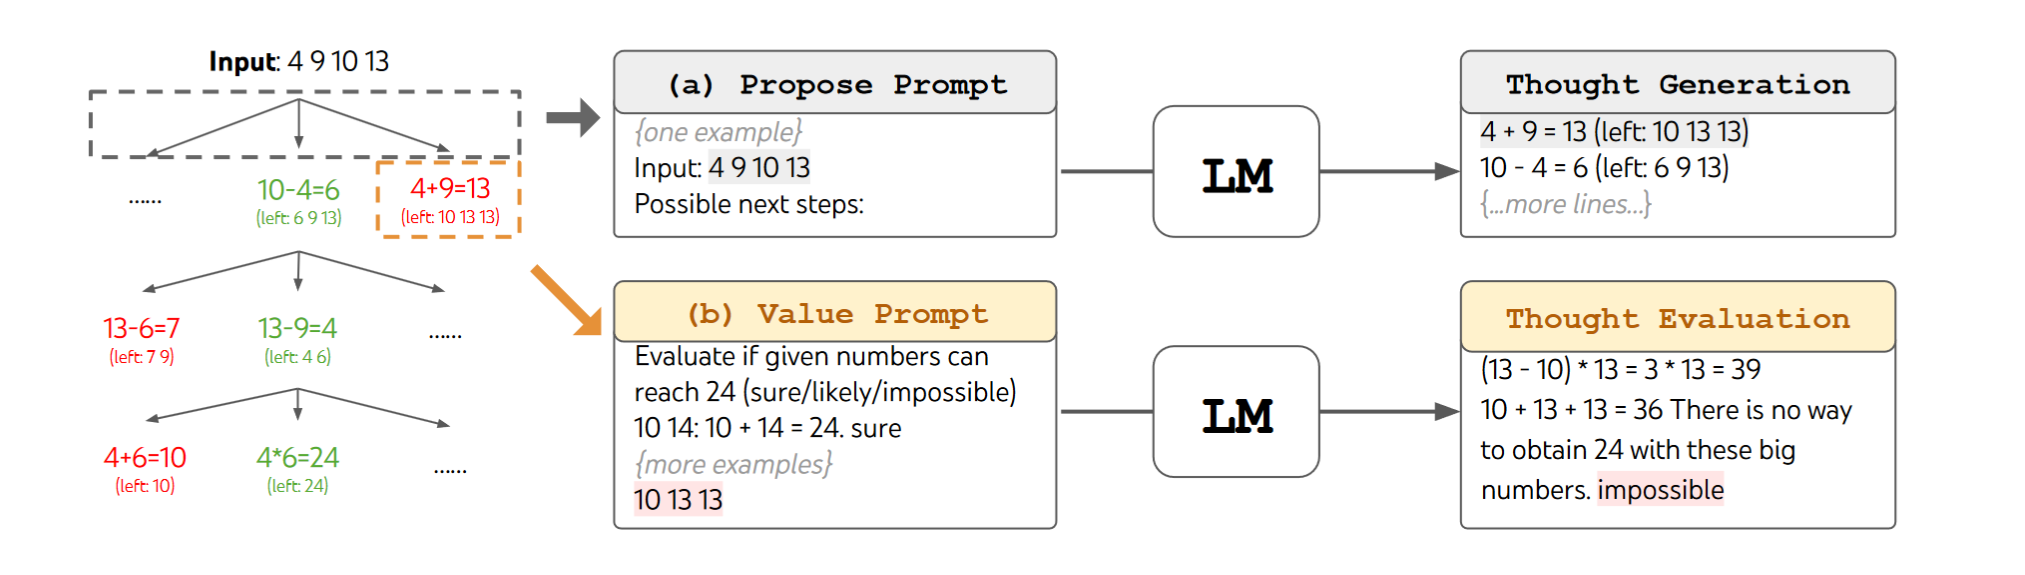
\includegraphics[width=0.99\textwidth]{game24sol.png} % Adjust width as needed
    \caption{ToT in a game of 24. The LM is prompted for (a) thought generation and (b) valuation.}
    \end{figure}
    
\end{frame}


\begin{frame}{limitations}
    \textbf{Resource Intensive:}\\
    \\
\begin{table}[h!]
\centering
\begin{tabular}{|l|c|c|c|}
\hline
\textbf{Game of 24} & \textbf{Generate/Prompt tokens} & \textbf{Cost per case} & \textbf{Success} \\ \hline
IO (best of 100)    & 1.8k / 1.0k                   & \$0.13                 & 33\%             \\ \hline
CoT (best of 100)   & 6.7k / 2.2k                   & \$0.47                 & 49\%             \\ \hline
ToT                 & 5.5k / 1.4k                   & \$0.74                 & 74\%             \\ \hline
\end{tabular}
\caption{Cost analysis on Game of 24.}
\end{table}

\textbf{Limited Applicability:}Limited to tasks requiring structured and logical problem-solving.
    
\end{frame}


\begin{frame}{Capabilities of ToT Framework}

\begin{itemize}
    \item \textbf{Enhanced Decision-Making.}
    
    \vspace{.5cm}
    \item \textbf{Applied primarily to reasoning and search problems.}
    
    
\end{itemize}

\end{frame}

\begin{frame}{}
    \centering
    {\Huge \textbf{Thank You!}}
    
\end{frame}


\end{document}